\part{Graph Traversals and Applications}
\label{ch:traversal}


\chapter{Graph traversal algorithms}

Traversals involve visiting each node of a digraph in a systematic way using only the structure of the digraph, that is, following only the arcs in the digraph. 
This is a very common task when dealing with digraphs and we'll cover several applications in later lectures.

%There are several ways to perform a systematic and efficient traversal.  
%We start with a basic framework for traversals then present the
%two most common techniques: breadth-first search and depth-first search.
%We also discuss a more general algorithm, priority-first search. 

\section{The general graph traversal algorithm}
\label{sec:trav}

All graph traversal algorithms  have the same basic structure  that relies on keeping track of which nodes have been visited and whether they may be adjacent to nodes that have not yet been visited. We use a system of three colours to to describe these states (see  \cref{fig:travcols}):
\begin{itemize} 
\item \defnfont{White nodes} have not yet been visited;
\item \defnfont{Grey nodes} (or \defnfont{frontier nodes}) have been visited but may have 
 out-neighbours that are white;
\item \defnfont{Black nodes} have been visited and all their out-neighbours have been visited too (so are not white). 
\end{itemize}
\begin{figure}
  \centering
  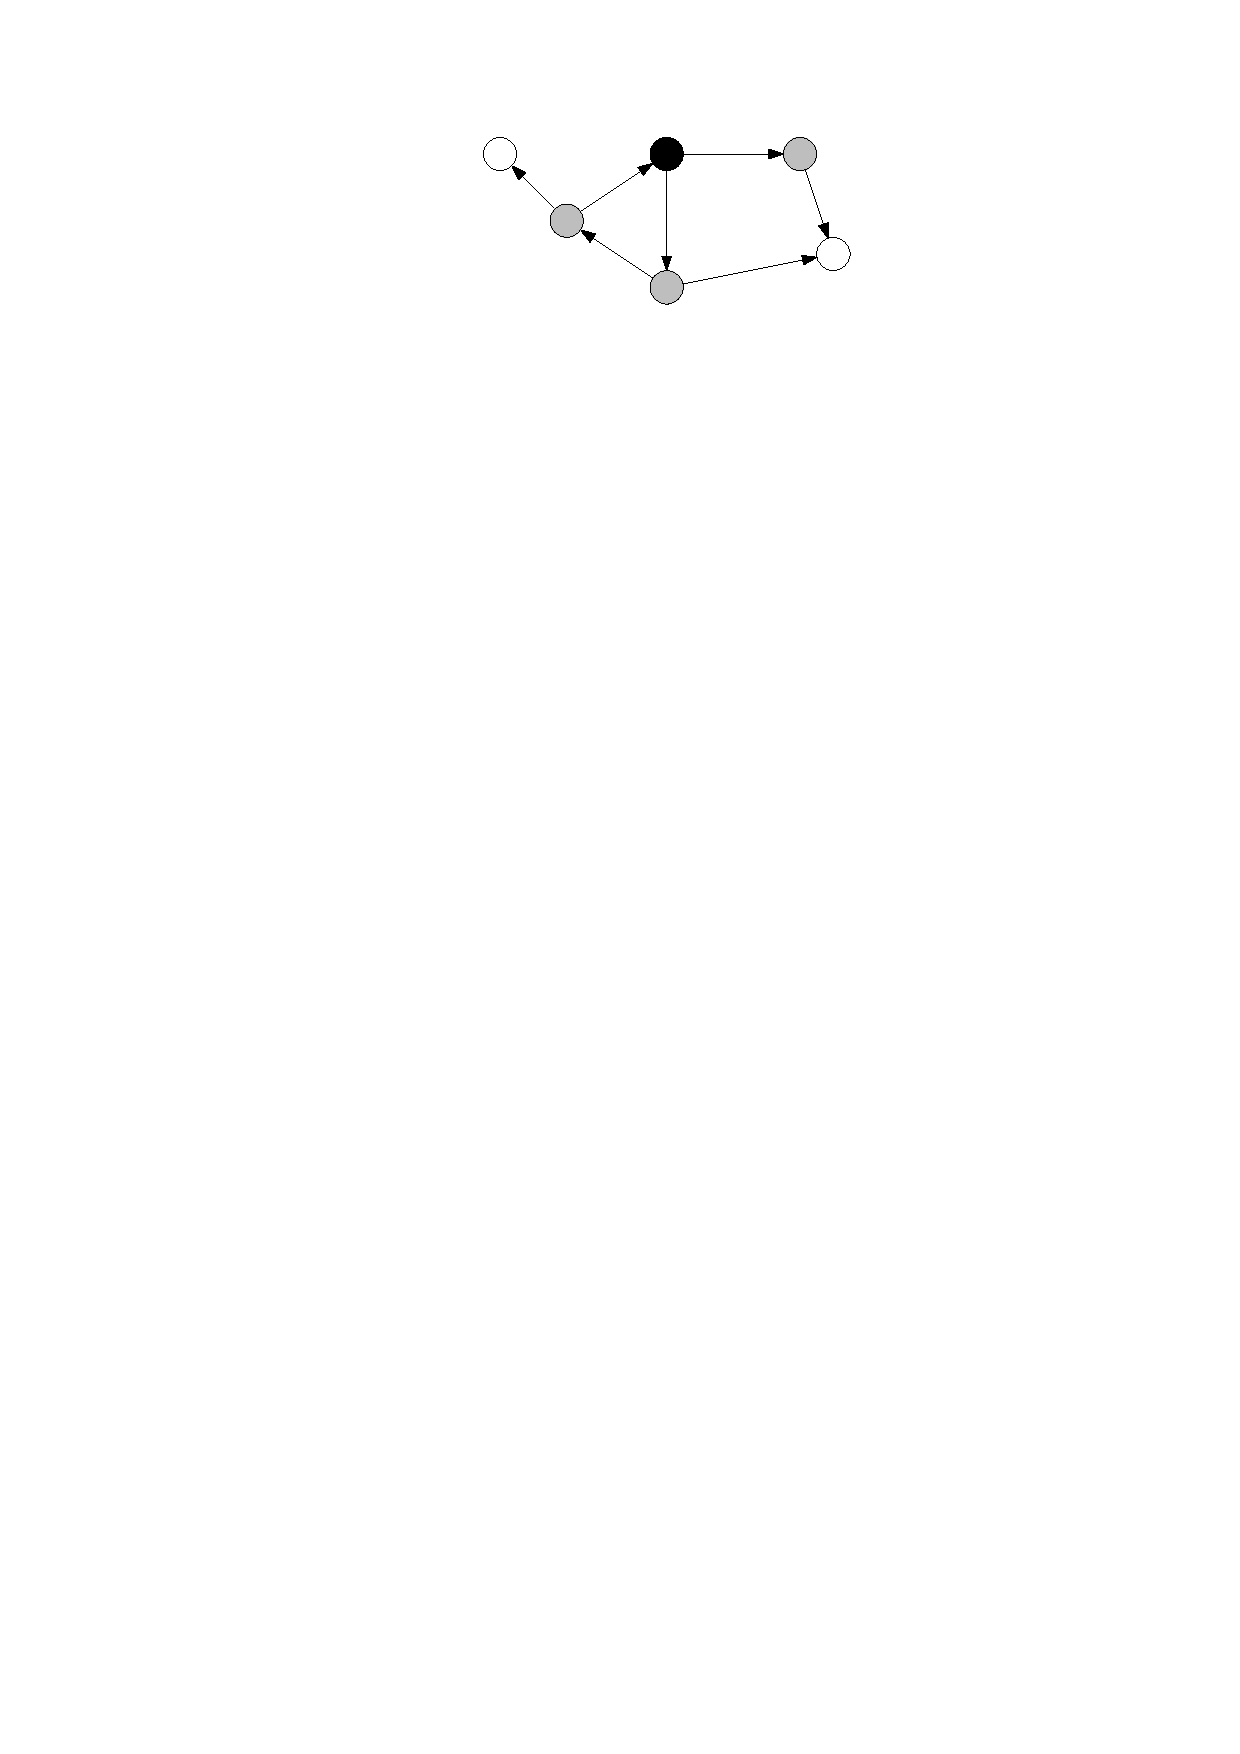
\includegraphics{graphTraversalNodeStateBW}
  \caption{Node states during a digraph traversal.}
  \label{fig:travcols}
\end{figure}


The traversal algorithm which visits all nodes in a digraph is loosely described as follows: 
\begin{itemize}
\item all nodes are white to begin with
\item a starting white node is chosen and turned grey
\item a grey node is chosen and its out-neighbours explored. 
\item If any out-neighbour is white, it is visited and turned grey. If no out-neighbours are white, the grey node is turned black. 
\item the process of choosing grey nodes and exploring neighbours is continued until all nodes reachable from the initial node are black.
\item if any white nodes remain in the digraph, a new  starting node is chosen and the process continues until all nodes are black.
\end{itemize}

We keep track of the order in which nodes are visited by recording which arc was followed when a node first turned from white to grey. As we will see, this creates a sub-digraph of the original digraph which has a tree structure.

The traversal algorithm is formalised in the pseudocode  of \cref{alg:traverse,alg:visit}. \cref{alg:traverse} (\algfont{traverse}) initialises the process and is tasked with finding white nodes to start from. Most of the work is done in \cref{alg:visit} (\algfont{visit}) which takes a starting node and explores the portion of the subgraph reachable from that node.

\begin{algorithm}[H]
  \caption{Basic graph traversal main routine: traverse
    \label{alg:traverse}}
\begin{algorithmic}[1]
\Function{traverse}{digraph $G$}
	\State  array $\colour[0..n-1]$ \Comment{records node colour}
	\State array $\pred[0..n-1]$ \Comment{records path of traversal as a tree}
	\For{$u \in V(G)$} \Comment{make all nodes white}
		\State $\colour[u] \gets $ WHITE 
	\EndFor
	\For{$s \in V(G)$}  \Comment{find a white node}
		\If {$\colour[s] ==$ WHITE} 
			\State \texttt{visit}$[s]$ \Comment{start traversal from $s$}
		\EndIf
	\EndFor
	\Return $\pred$ 
\EndFunction
\end{algorithmic}
\end{algorithm}

\begin{algorithm}[H]
  \caption{Basic graph traversal subroutine: visit
    \label{alg:visit}}
\begin{algorithmic}[1]
\Function{visit}{node $s$ of digraph $G$}
	\State  $\colour[s] \gets$ GREY 
	\State $\pred[s] \gets$ NULL \Comment{make start node the root of the tree}
	\While{there is a GREY node} \Comment{continues until all nodes are black}
		\State choose a GREY node $u$ 
		\If{$u$ has a WHITE neighbour}
			\State choose a WHITE neighbour, $v$ 
			\State $\colour[v] \gets $ GREY \Comment{$v$ is visited for first time, so turns grey }
			\State $pred[v] \gets u$ \Comment{make $u$ the parent of $v$ in the traversal tree}
		\Else
			\State $\colour[u] \gets $ BLACK \Comment{$u$ has no white neighbours so done with $u$ }
		\EndIf
	\EndWhile
\EndFunction
\end{algorithmic}
\end{algorithm}

After the first call to \algfont{visit} we have created a subdigraph of $G$ that is a tree: the
nodes are precisely the black nodes (all nodes reachable from the initial node), and the arcs are those arcs followed when we found a white neighbour of a grey node. 

Each white node chosen in \algfont{traverse} becomes the root of a tree in the call to \algfont{visit}. Eventually, we obtain a
set of disjoint trees spanning the digraph (that is, it includes all the nodes of the digraph), which we call the
\defnfont{search forest}. The search forest  is returned by \algfont{traverse} in the array $pred$.

\tikz{
\foreach \x/\y/\c in {3/2/a,0/0/b,1/2/c,2/-2/d,4/0/e} {
     \draw[blue,thick] (\x,\y) circle(3mm) node[black] {\footnotesize\c};
}
\draw[blue,thick,-latex] (0.135,0.27) -- (0.865,1.73); %b->c
\draw[blue,thick,-latex] (0.25,0.167) -- (2.75,1.833); %b->a
\draw[blue,thick,-latex] (3.135,1.73) -- (3.865,0.27); %a->e
\draw[blue,thick,-latex] (1.3,2) -- (2.7,2);  %c->a
\draw[blue,thick,-latex] (1.073,1.708) -- (1.927,-1.708); %c->d   
\draw[blue,thick,-latex] (1.788,-1.788) -- (0.212,-0.212); %d->b  
\draw[blue,thick,-latex] (2.212,-1.788) -- (3.788,-0.212); %d->e
\node[below] at (8,2) {\begin{minipage}{60mm} \footnotesize
initialising all nodes WHITE\\
\end{minipage}};
}


\tikz{
\foreach \x/\y/\c in {3/2/a,0/0/b,1/2/c,2/-2/d,4/0/e} {
     \draw[blue,thick] (\x,\y) circle(3mm) node[black] {\footnotesize\c};
}
\draw[blue,thick,-latex] (0.135,0.27) -- (0.865,1.73); %b->c
\draw[blue,thick,-latex] (0.25,0.167) -- (2.75,1.833); %b->a
\draw[blue,thick,-latex] (3.135,1.73) -- (3.865,0.27); %a->e
\draw[blue,thick,-latex] (1.3,2) -- (2.7,2);  %c->a
\draw[blue,thick,-latex] (1.073,1.708) -- (1.927,-1.708); %c->d   
\draw[blue,thick,-latex] (1.788,-1.788) -- (0.212,-0.212); %d->b  
\draw[blue,thick,-latex] (2.212,-1.788) -- (3.788,-0.212); %d->e
\foreach \x/\y/\c/\d in {3/2/a/very thick,4/0/e/ultra thick} {
     \filldraw[black!25] (\x,\y) circle (3mm);
     \draw[blue,\d] (\x,\y) circle(3mm) node[black] {\footnotesize\c};
}
\node[below] at (8,2) {\begin{minipage}{60mm} \footnotesize
\texttt{visit}(a); $colour[\textsf{a}]\leftarrow\textsf{GREY}$\\
e is  WHITE neighbour of a:\\
\hspace*{4mm} $colour[\textsf{e}]\leftarrow\textsf{GREY}$; $pred[\textsf{e}]\leftarrow\textsf{a}$\\
\end{minipage}};
}

\tikz{
\foreach \x/\y/\c in {3/2/a,0/0/b,1/2/c,2/-2/d,4/0/e} {
     \draw[blue,thick] (\x,\y) circle(3mm) node[black] {\footnotesize\c};
}
\draw[blue,thick,-latex] (0.135,0.27) -- (0.865,1.73); %b->c
\draw[blue,thick,-latex] (0.25,0.167) -- (2.75,1.833); %b->a
\draw[blue,thick,-latex] (3.135,1.73) -- (3.865,0.27); %a->e
\draw[blue,thick,-latex] (1.3,2) -- (2.7,2);  %c->a
\draw[blue,thick,-latex] (1.073,1.708) -- (1.927,-1.708); %c->d   
\draw[blue,thick,-latex] (1.788,-1.788) -- (0.212,-0.212); %d->b 
\draw[blue,thick,-latex] (2.212,-1.788) -- (3.788,-0.212); %d->e
\foreach \x/\y/\c/\d in {3/2/a/very thick,4/0/e/ultra thick} {
     \filldraw[black!25] (\x,\y) circle (3mm);
     \draw[blue,\d] (\x,\y) circle(3mm) node[black] {\footnotesize\c};
}
\filldraw[black] (3,2) circle (2.9mm) node[yellow] {\footnotesize a};
\node[below] at (8,2) {\begin{minipage}{60mm} \footnotesize
\texttt{visit}(a); $colour[\textsf{a}]\leftarrow\textsf{GREY}$\\
e is  WHITE neighbour of a\\
\hspace*{4mm} $colour[\textsf{e}]\leftarrow\textsf{GREY}$; $pred[e]\leftarrow\textsf{a}$\\
choose GREY a: {\footnotesize no WHITE neighbour:} \\
\hspace*{4mm}$colour[\textsf{a}]\leftarrow\textsf{BLACK}$\\
\end{minipage}};
}



\tikz{
\foreach \x/\y/\c in {3/2/a,0/0/b,1/2/c,2/-2/d,4/0/e} {
     \draw[blue,thick] (\x,\y) circle(3mm) node[black] {\footnotesize\c};
}
\draw[blue,thick,-latex] (0.135,0.27) -- (0.865,1.73); %b->c
\draw[blue,thick,-latex] (0.25,0.167) -- (2.75,1.833); %b->a
\draw[blue,thick,-latex] (3.135,1.73) -- (3.865,0.27); %a->e
\draw[blue,thick,-latex] (1.3,2) -- (2.7,2);  %c->a
\draw[blue,thick,-latex] (1.073,1.708) -- (1.927,-1.708); %c->d   
\draw[blue,thick,-latex] (1.788,-1.788) -- (0.212,-0.212); %d->b 
\draw[blue,thick,-latex] (2.212,-1.788) -- (3.788,-0.212); %d->e
\foreach \x/\y/\c/\d in {3/2/a/very thick,4/0/e/ultra thick} {
     \filldraw[black!25] (\x,\y) circle (3mm);
     \draw[blue,\d] (\x,\y) circle(3mm) node[black] {\footnotesize\c};
}
\filldraw[black] (3,2) circle (2.9mm) node[yellow] {\footnotesize a};
\filldraw[black] (4,0) circle (2.9mm) node[yellow] {\footnotesize e};
\node[below] at (8,2) {\begin{minipage}{60mm} \footnotesize
\texttt{visit}(a); $colour[\textsf{a}]\leftarrow\textsf{GREY}$\\
e is  WHITE neighbour of a\\
\hspace*{4mm} $colour[\textsf{e}]\leftarrow\textsf{GREY}$; $pred[e]\leftarrow\textsf{a}$\\
choose GREY a: {\footnotesize no WHITE neighbour:} \\
\hspace*{4mm}$colour[\textsf{a}]\leftarrow\textsf{BLACK}$\\
choose GREY e: {\footnotesize no WHITE neighbour:} \\
\hspace*{4mm}$colour[\textsf{e}]\leftarrow\textsf{BLACK}$\\
\end{minipage}};
}


\tikz{
\foreach \x/\y/\c in {3/2/c,0/0/a,1/2/b,2/-2/d,4/0/e} {
     \draw[blue,thick] (\x,\y) circle(3mm) node[black] {\footnotesize\c};
}
\draw[blue,thick,-latex] (0.135,0.27) -- (0.865,1.73); %b->c
\draw[blue,thick,-latex] (0.25,0.167) -- (2.75,1.833); %b->a
\draw[blue,thick,-latex] (3.135,1.73) -- (3.865,0.27); %a->e
\draw[blue,thick,-latex] (1.3,2) -- (2.7,2);  %c->a
\draw[blue,thick,-latex] (1.073,1.708) -- (1.927,-1.708); %c->d   
\draw[blue,thick,-latex] (1.788,-1.788) -- (0.212,-0.212); %d->b  
\draw[blue,thick,-latex] (2.212,-1.788) -- (3.788,-0.212); %d->e
\foreach \x/\y/\c/\d in {3/2/a/very thick,4/0/e/ultra thick,0/0/b/very thick,1/2/c/ultra thick} {
     \filldraw[black!25] (\x,\y) circle (3mm);
     \draw[blue,\d] (\x,\y) circle(3mm) node[black] {\footnotesize\c};
}
\filldraw[black] (3,2) circle (2.9mm) node[yellow] {\footnotesize a};
\filldraw[black] (4,0) circle (2.9mm) node[yellow] {\footnotesize e};
\node[below] at (8,2) {\begin{minipage}{60mm} \footnotesize
\texttt{visit}(b); $colour[\textsf{b}]\leftarrow\textsf{GREY}$\\
c is  WHITE neighbour of b\\
\hspace*{4mm} $colour[\textsf{c}]\leftarrow\textsf{GREY}$; $pred[c]\leftarrow\textsf{b}$\\
\end{minipage}};
}



\tikz{
\foreach \x/\y/\c in {3/2/c,0/0/a,1/2/b,2/-2/d,4/0/e} {
     \draw[blue,thick] (\x,\y) circle(3mm) node[black] {\footnotesize\c};
}
\draw[blue,thick,-latex] (0.135,0.27) -- (0.865,1.73); %b->c
\draw[blue,thick,-latex] (0.25,0.167) -- (2.75,1.833); %b->a
\draw[blue,thick,-latex] (3.135,1.73) -- (3.865,0.27); %a->e
\draw[blue,thick,-latex] (1.3,2) -- (2.7,2);  %c->a
\draw[blue,thick,-latex] (1.073,1.708) -- (1.927,-1.708); %c->d   
\draw[blue,thick,-latex] (1.788,-1.788) -- (0.212,-0.212); %d->b  
\draw[blue,thick,-latex] (2.212,-1.788) -- (3.788,-0.212); %d->e
\foreach \x/\y/\c/\d in {3/2/a/very thick,4/0/e/ultra thick,0/0/b/very thick,1/2/c/very thick,2/-2/d/ultra thick} {
     \filldraw[black!25] (\x,\y) circle (3mm);
     \draw[blue,\d] (\x,\y) circle(3mm) node[black] {\footnotesize\c};
}
\filldraw[black] (3,2) circle (2.9mm) node[yellow] {\footnotesize a};
\filldraw[black] (4,0) circle (2.9mm) node[yellow] {\footnotesize e};
\node[below] at (8,2) {\begin{minipage}{60mm} \footnotesize
\texttt{visit}(b); $colour[\textsf{b}]\leftarrow\textsf{GREY}$\\
c is  WHITE neighbour of b\\
\hspace*{4mm} $colour[\textsf{c}]\leftarrow\textsf{GREY}$; $pred[c]\leftarrow\textsf{b}$\\
d is WHITE neighbour of c\\
\hspace*{4mm} $colour[\textsf{d}]\leftarrow\textsf{GREY}$; $pred[d]\leftarrow\textsf{c}$\\
\end{minipage}};
}

\tikz{
\foreach \x/\y/\c in {3/2/c,0/0/a,1/2/b,2/-2/d,4/0/e} {
     \draw[blue,thick] (\x,\y) circle(3mm) node[black] {\footnotesize\c};
}
\draw[blue,very thick,-latex] (0.135,0.27) -- (0.865,1.73); %b->c
\draw[blue,thick,dashed,-latex] (0.25,0.167) -- (2.75,1.833); %b->a
\draw[blue,very thick,-latex] (3.135,1.73) -- (3.865,0.27); %a->e
\draw[blue,thick,dashed,-latex] (1.3,2) -- (2.7,2);  %c->a
\draw[blue,very thick,-latex] (1.073,1.708) -- (1.927,-1.708); %c->d   
\draw[blue,thick,dashed,-latex] (1.788,-1.788) -- (0.212,-0.212); %d->b  
\draw[blue,thick,dashed,-latex] (2.212,-1.788) -- (3.788,-0.212); %d->e
\foreach \x/\y/\c/\d in {3/2/a/very thick,4/0/e/ultra thick,0/0/b/very thick,1/2/c/very thick,2/-2/d/ultra thick} {
     \filldraw[black] (\x,\y) circle (3mm);
     \draw[blue,\d] (\x,\y) circle(3mm) node[yellow] {\footnotesize\c};
}
\node[below] at (8,2) {\begin{minipage}{60mm} \footnotesize
\texttt{visit}(b); $colour[\textsf{b}]\leftarrow\textsf{GREY}$\\
c is  WHITE neighbour of b\\
\hspace*{4mm} $colour[\textsf{c}]\leftarrow\textsf{GREY}$; $pred[c]\leftarrow\textsf{b}$\\
d is WHITE neighbour of c\\
\hspace*{4mm} $colour[\textsf{d}]\leftarrow\textsf{GREY}$; $pred[d]\leftarrow\textsf{c}$\\
no more WHITE nodes:\\
\hspace*{4mm} $colour[\textsf{d}]\leftarrow\textsf{BLACK}$\\
\hspace*{4mm} $colour[\textsf{c}]\leftarrow\textsf{BLACK}$\\
\hspace*{4mm} $colour[\textsf{b}]\leftarrow\textsf{BLACK}$\\
\end{minipage}};
} 


\section{Classifying arcs after a traversal}

For the analysis of the traversal algorithm, it is useful to classify the arcs of $G$ based on their relationships in the search forest.  

\begin{Definition}\label{defn:arc-types}
Suppose we have performed a traversal of a digraph $G$, resulting in a
search forest $F$.  Let $(u, v)\in E(G)$ be an arc. Then $(u, v)$ is a:
\begin{itemize} 
\item \defnfont{tree arc} if it belongs to one of the trees of $F$. 
\item Or, if it is not a tree arc, it is a
\begin{itemize}
\item \defnfont{forward arc} if $u$ is an ancestor of $v$ in $F$
\item \defnfont{back arc} if $u$ is a descendant of $v$ in $F$
\item \defnfont{cross arc} if neither $u$ nor $v$ is an ancestor of the other in $F$.
\end{itemize}
\end{itemize}
\end{Definition} 

A cross arc may 
join two nodes in the same tree or point from one tree to another in the search forest. Tree, forward and back arcs require that $u$ and $v$ be in the same tree.



\tikz{
\foreach \x/\y/\c in {3/2/c,0/0/a,1/2/b,2/-2/d,4/0/e} {
     \draw[blue,thick] (\x,\y) circle(3mm) node[black] {\footnotesize\c};
}
\draw[blue,very thick,-latex] (0.135,0.27) -- (0.865,1.73); %b->c
\draw[thick,dashed,-latex] (0.25,0.167) -- (2.75,1.833); %b->a
\draw[blue,very thick,-latex] (3.135,1.73) -- (3.865,0.27); %a->e
\draw[thick,dashed,-latex] (1.3,2) -- (2.7,2);  %c->a
\draw[blue,very thick,-latex] (1.073,1.708) -- (1.927,-1.708); %c->d   
\draw[magenta,thick,dashed,-latex] (1.788,-1.788) -- (0.212,-0.212); %d->b  
\draw[thick,dashed,-latex] (2.212,-1.788) -- (3.788,-0.212); %d->e
\foreach \x/\y/\c/\d in {3/2/a/very thick,4/0/e/ultra thick,0/0/b/very thick,1/2/c/very thick,2/-2/d/ultra thick} {
     \filldraw[black] (\x,\y) circle (3mm);
     \draw[blue,\d] (\x,\y) circle(3mm) node[yellow] {\footnotesize\c};
}
}


The following theorem collects all the basic facts we need for proofs
in later sections. The proofs are simple and can be done as exercises. %\cref{fig:travdecomp} illustrates the first part.

\begin{Theorem}
\label{thm:trav}
Suppose that we have carried out \algfont{traverse} on $G$, 
resulting in a search forest $F$. Let $v, w \in V(G)$.
\begin{itemize}
\item Let $T_1$ and $T_2$ be different trees in $F$ and suppose that $T_1$ was 
explored before $T_2$. Then there are no arcs from $T_1$ to $T_2$. 

\item Suppose that $G$ is a graph. Then there can be no edges joining different 
trees of $F$.

\item Suppose that $v$ is visited before $w$ and $w$ is reachable from $v$ in 
$G$. Then $v$ and $w$ belong to the same tree of $F$.

\item Suppose that $v$ and $w$ belong to the same tree $T$ in $F$. Then any path
 from $v$ to $w$ in $G$ must have all nodes in $T$.
\end{itemize}
\end{Theorem}

%\begin{proof}
%If the first part were not true, then since $w$ is reachable from $v$,
%and $w$ has not been visited before $T_1$ is started, $w$ must be reached
%in the generation of $T_1$, contradicting $w\in T_2$. The second part
%follows immediately for symmetric digraphs and hence for graphs. Now
%suppose that $v$ is seen before $w$. Let $r$ be the root of the tree $T$
%containing $v$. Then $w$ is reachable from $r$ and so since it has not
%already been visited when $r$ is chosen, it belongs to $T$. Finally, if
%$v$ and $w$ are in the same tree, then any path from $v$ to $w$ in $G$
%going outside the tree must re-enter it via some arc; either the leaving
%or the entering arc will contradict the first part.
%\end{proof}

\begin{Boxample}[2]
Assuming the first statement, prove the third statement
\end{Boxample}

%\begin{figure}[htbp]
%  \centering
%  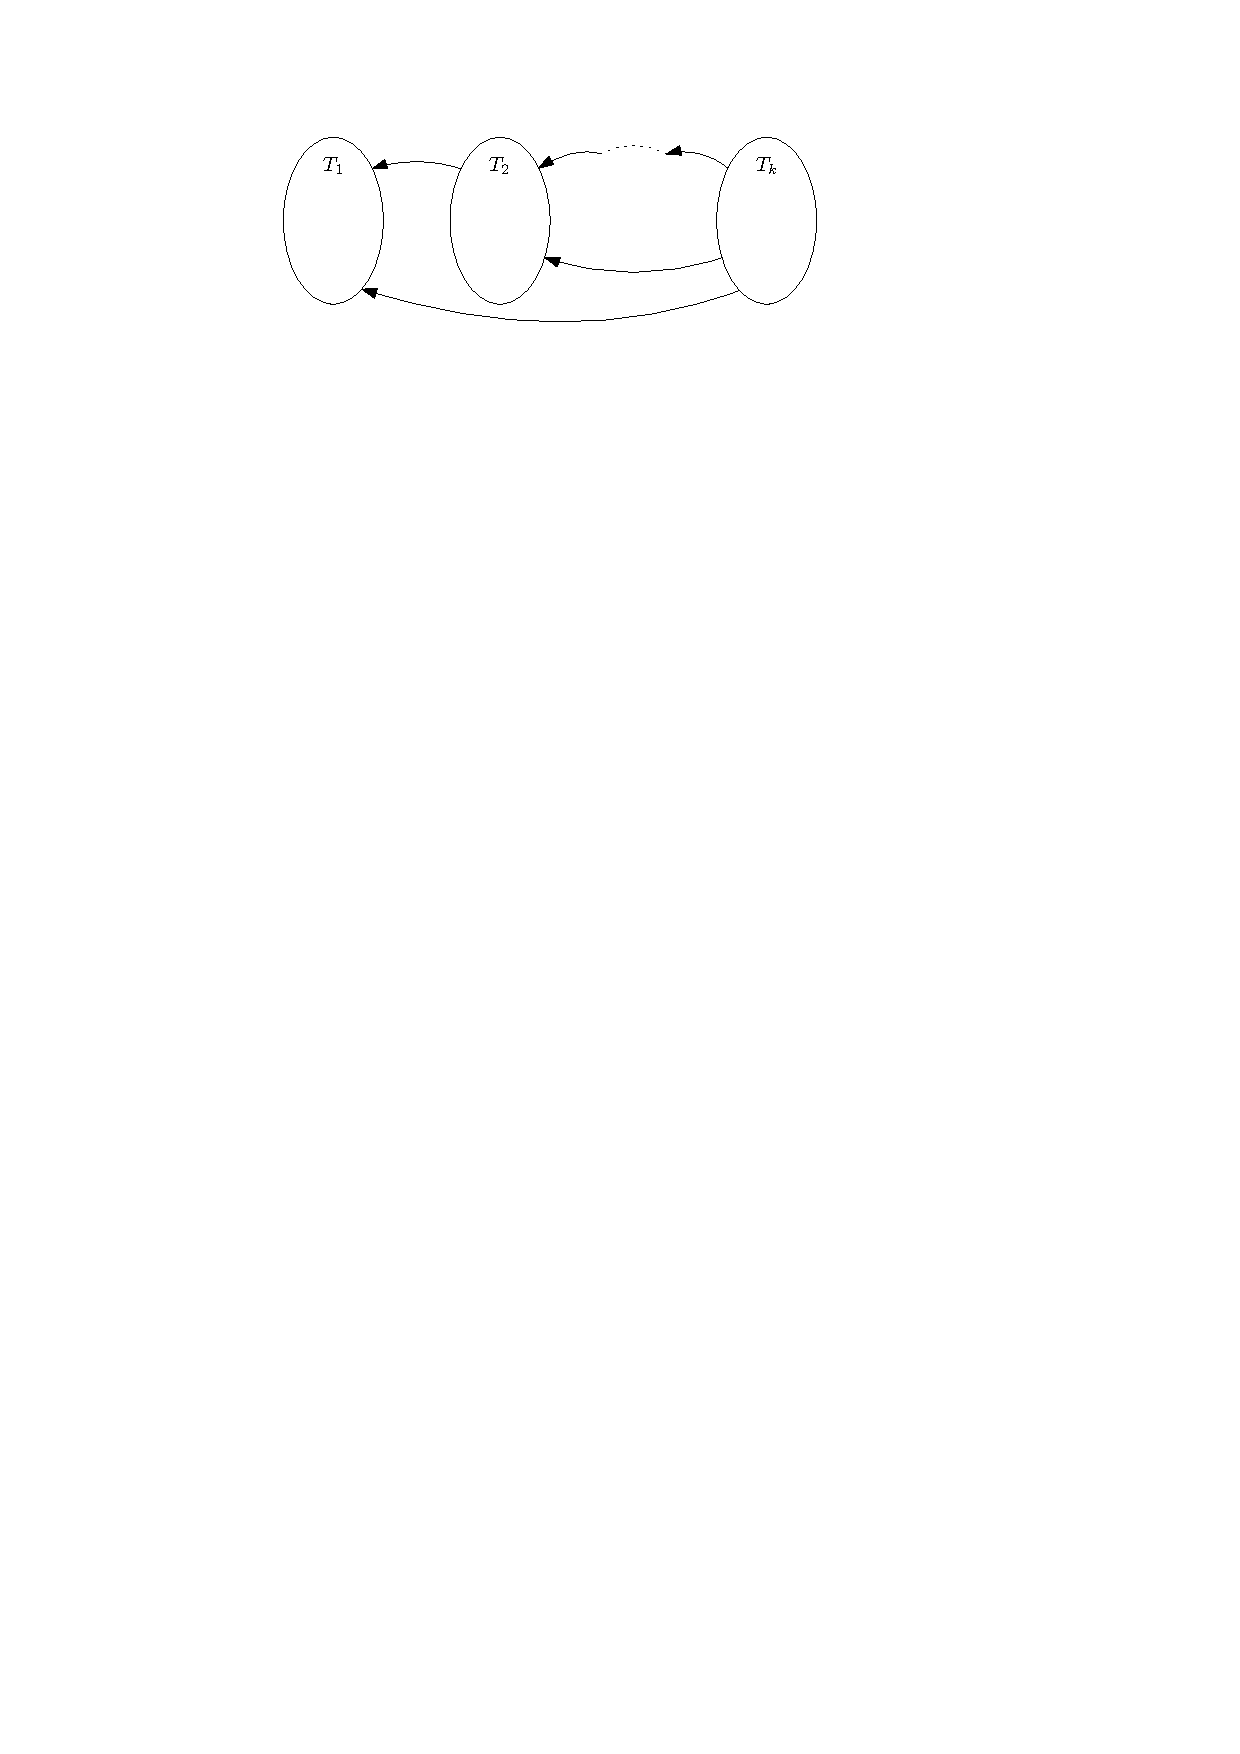
\includegraphics{decomposition}
%  \caption{Decomposition of a digraph in terms of search trees.}
%  \label{fig:travdecomp}
%\end{figure}

\section{Running time for the general traversal algorithm}

The generality
of our traversal algorithm makes it exact running time impossible to determine.  It depends on how one chooses the next grey node $u$
and its white neighbour $v$.  SOme schemes for choosing $u$ and $v$ can be complex and depend on $n$. Here consider that the schemes are simple and constant time. 

%It also apparently depends on how long it
%takes to determine whether there exist any grey nodes or whether $u$ has
%any white neighbours. However, any sensible rule for checking existence
%of either type of node should simply return false if there is no such
%node, and take no more time in this case than if it does find one. Thus
%we do not need to take account of the checking in our analysis.

\begin{itemize}
\item The initialization of the array $\colour$ takes time 
$\Theta(n)$ so \algfont{traverse} 
is in $\Theta(n + t)$, where $t$ is the total time taken by all 
the calls to \algfont{visit}.

%Each time through the while-loop a grey node is
%chosen, and either a white node is turned grey or a grey node is turned
%black. Note that the same grey node can be chosen many times. Thus
\item We execute the while-loop of \algfont{visit} in total $\Theta(n)$ times since every node
must eventually move from white through grey to black. 

\item The time taken in choosing grey nodes is
$\Omega(n)$. 

\item The time taken to find a white neighbour involves examining each  neighbour of $u$ and checking whether it is
white, then applying a selection rule. 

\item  the total 
time in
choosing white neighbours $\Omega(m)$ if adjacency lists
are used and $\Omega(n^2)$ if an adjacency matrix is used.

\item So the running time of \algfont{traverse} is $\Omega(n + (n+m)) = \Omega(n + m)$
if adjacency lists are used, and $\Omega(n + n^2) = \Omega(n^2)$ if adjacency matrix format is used.

\end{itemize}

So for simple selection rules and assuming a sparse input digraph, the adjacency list format seems
preferable. 

But if more complex selection rules are used, for example, choosing a single grey node is 
of order $n$ while choosing a single white node is still constant time, then running time is 
asymptotically $\Omega(n^2)$ regardless of the data structure, so using
the adjacency matrix is not clearly ruled out.

%\subsection*{Exercises}
%
%\begin{Exercise}
%\label{ex:trav-maze}
%Draw a moderately complicated graph representing a maze (corridors are
%edges and intersections are nodes). Label one node as the start and
%another as the end.  One rule for getting through a maze is to  try to
%go forward, always make a right turn when faced with a choice of
%direction, and back up as little as possible when faced with a dead end.
%Apply this method to your example. Interpret what you do in terms of the
%procedure \algfont{traverse}.
%\end{Exercise}
%
%\begin{Exercise}
%\label{ex:trav-maze-random}
%Suppose that in \algfont{traverse}, the grey node is chosen at random and
%so is the white node. Find your way through your maze of the previous
%exercise using this method.
%\end{Exercise}
%
%\begin{Exercise}
%\label{ex:trav-cross}
%Give an example for each of the following items.
%\begin{itemize}
%\item A search forest in which a cross arc points from one tree to 
%another.
%\item A  search forest in which a cross arc joins two nodes in the same
%tree.
%\end{itemize}
%\end{Exercise}

\chapter{Depth first search }

Traversal algorithms differ in the rules for choosing the next grey and next white node, with  different rules lead
to very different results.  Here we

\begin{itemize}
\item in \defnfont{depth-first
search} (DFS) the new grey node chosen is the one
that has been grey for the \boldfont{shortest} time
\end{itemize}
 
%BFS takes us away
%from the root node as slowly as possible. First we visit the root, then all its neighbours, then all neighbours of its neighbours and so on. The root is the first node to turn black.

%By contrast, 

DFS  takes us away
from the root node as quickly as possible. If the first visited neighbour of the root has a neighbour, we immediately visit that neighbour. Then, it that has a neighbour , we visit that and so on, thus ``deeply''
searching as far away from the root as possible. We backtrack as little as possible before continuing away from the root again. The root is the last node to turn black.

There still remains the choice
of which white neighbour of the chosen grey node to visit. It does
not matter what choice is made but our \defnfont{convention is to choose the one with
lowest index} (recall nodes have indices $0, \dots, n - 1$). 

These choices can be made in constant time so that the running time is  $\Omega(n + m)$ (assuming adjacency lists). So DFS are linear in the size + order of a digraph. 

If an adjacency matrix is used, the algorithms are quadratic in the size of the graph ($\Omega(n^2)$).

\begin{Example}
\label{eg:graphExample2}
A graph $G_1$ and a digraph $G_2$ are displayed in
\cref{fig:graphExample2}.

In \cref{fig:graphEx2-DFS} we show the depth-first search trees based on a DFS traversal starting at node $0$. The
dashed arcs indicate the original arcs that are not part of the DFS trees.
\end{Example}



\begin{Boxample}[2]
Find a tree arc, cross arc, forward arc and back arc for each of the search trees in \cref{fig:graphEx2-DFS} (or say if that type of arc does not exist for that traversal).
\end{Boxample}


\begin{figure}[hbtp]
	\centering
	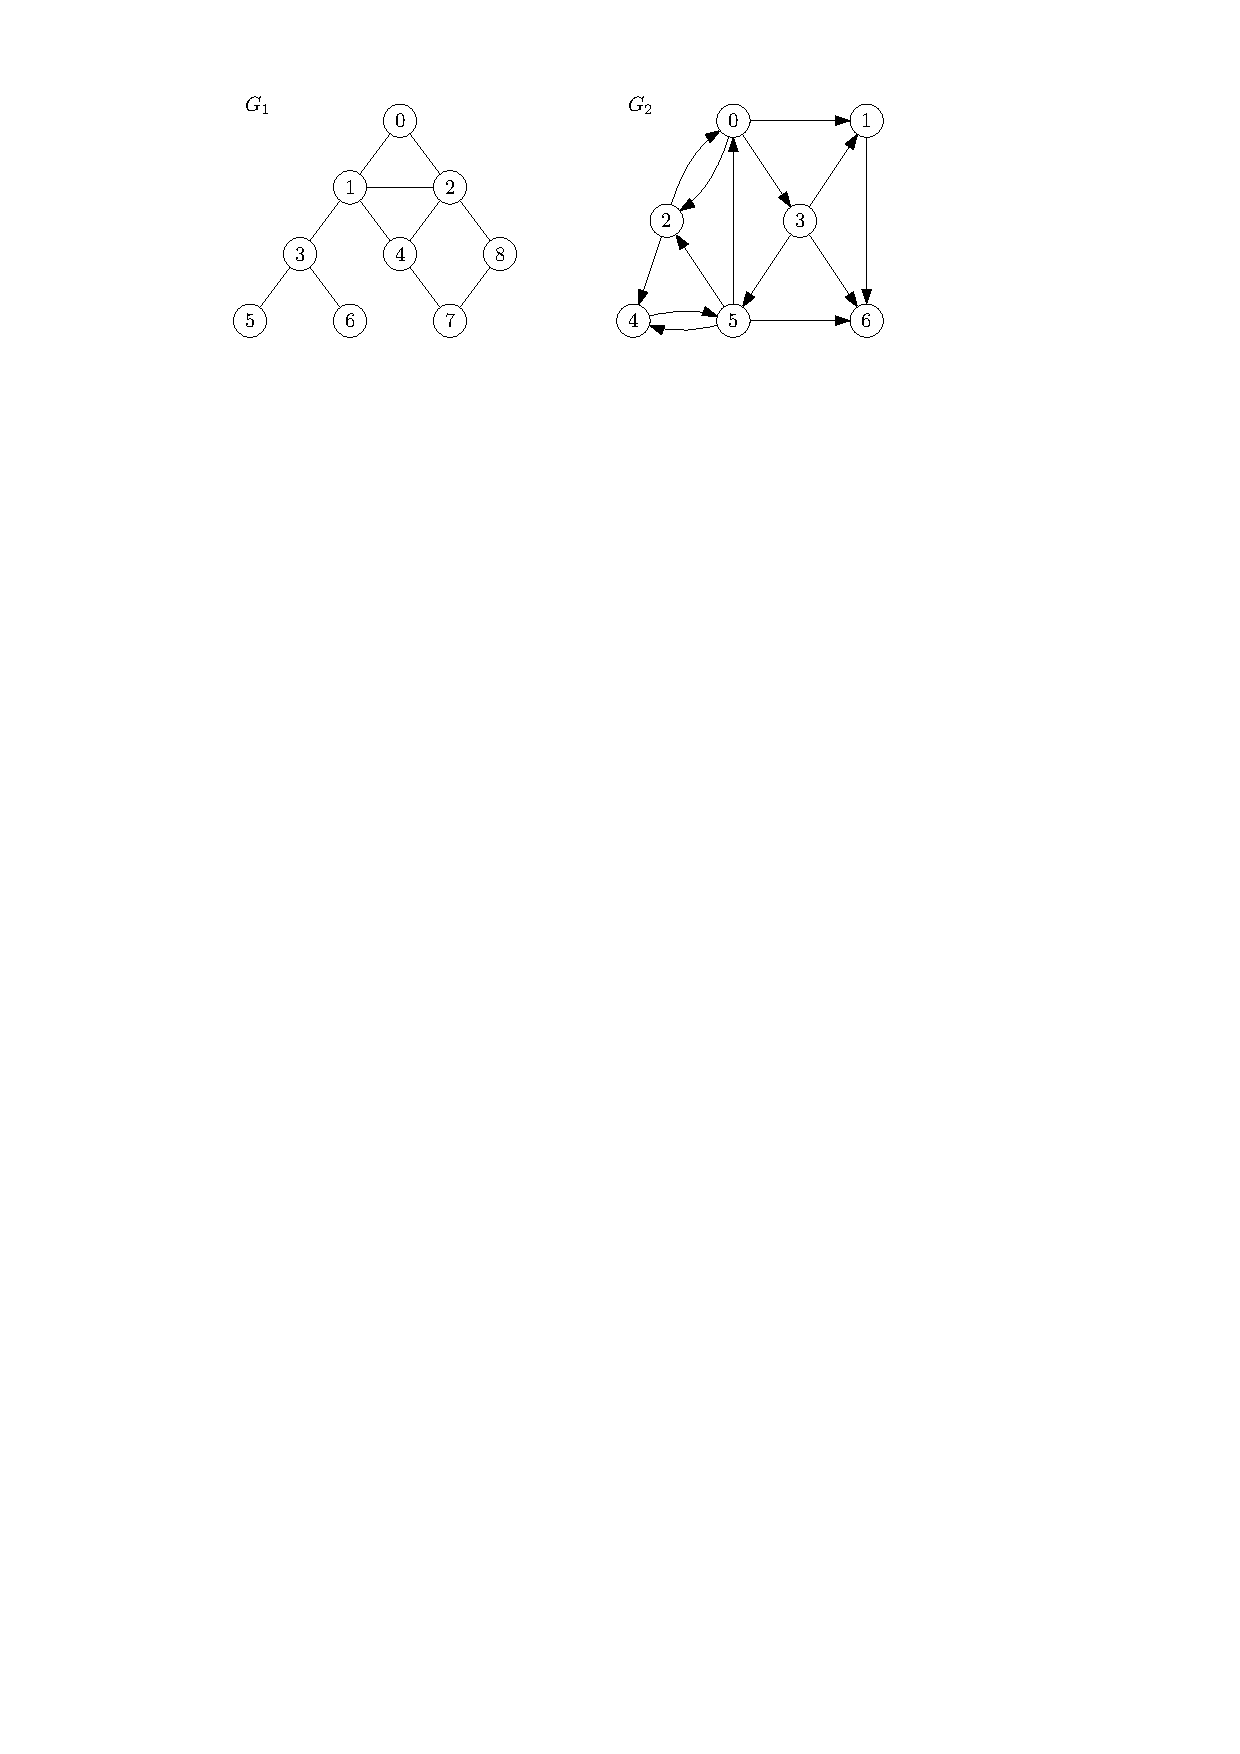
\includegraphics{graphEx2}
	\caption{A graph $G_1$ and a digraph $G_2$.}
	\label{fig:graphExample2}
\end{figure}



\begin{figure}[hbtp]
	\centering 
	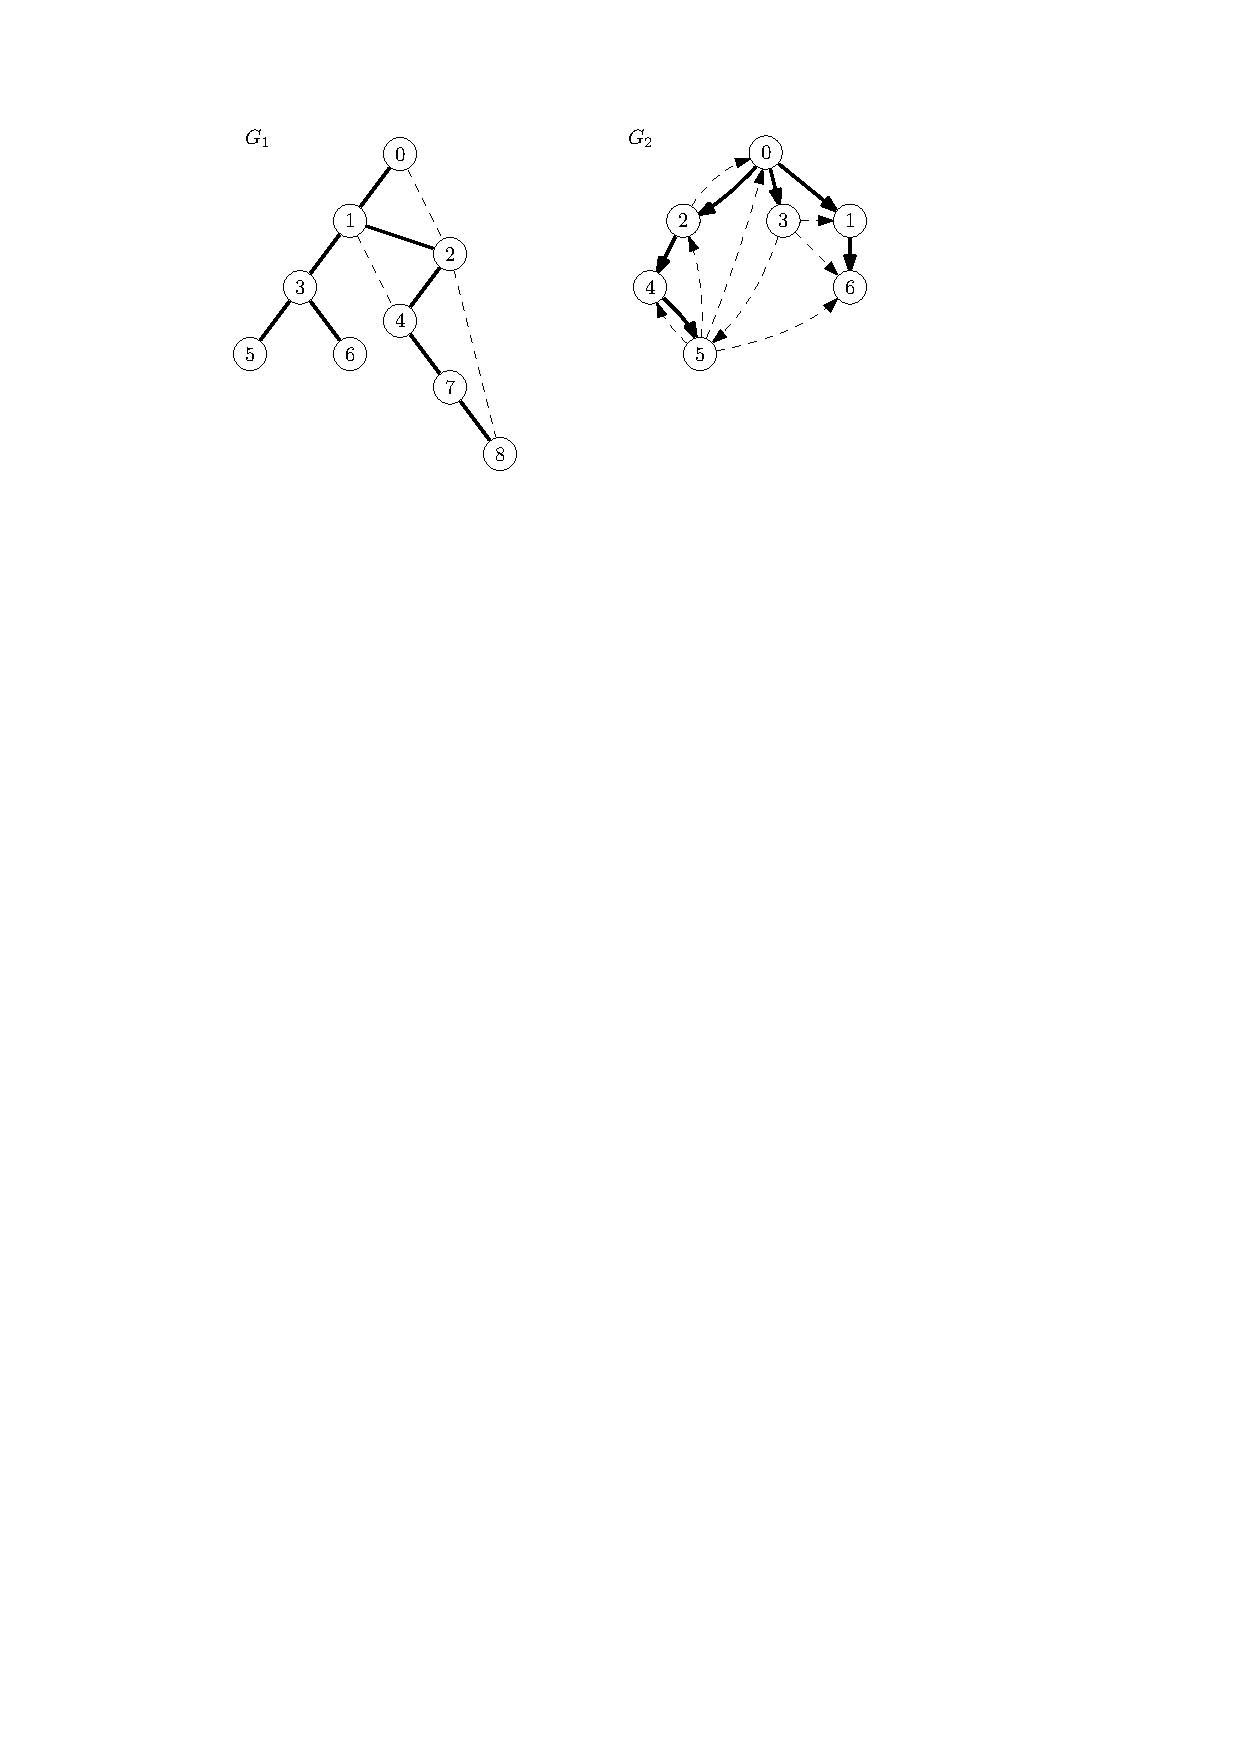
\includegraphics{graphEx2DFS}
	\caption{DFS trees for $G_1$ and $G_2$, rooted at $0$.}
	\label{fig:graphEx2-DFS}
\end{figure}

For a general digraph, and unlike the examples given here, all nodes may not be reachable from the starting node. In this case, each call to \algfont{DFSvisit} (a special case of \algfont{visit}) produces a single search tree, while the algorithm \algfont{DFS} (a special case of \algfont{traverse}) repeatedly chooses a root and runs the associated visit algorithm, producing the search forest.

%\section*{Exercises}
%
%\begin{Exercise}
%\label{exr:bfs-vs-dfs}
%Draw a graph for which DFS and BFS can visit nodes in the same order. Then 
%draw one for which they must visit nodes in the same order. Make your examples 
%as large as possible (maximize $n+m$).
%\end{Exercise}
%
%\begin{Exercise}
%\label{exr:iterative-deep}
%A technique called \defnfont{iterative deepening} combines features of BFS and DFS.
%Starting at a root, for each $i = 0, 1, \dots$ we search all nodes at distance 
%at most $i$, using DFS (in other words, we limit the depth of the DFS to $i$). 
%We do this for each $i$ until the whole graph is explored or we reach a 
%preassigned limit on $i$.
%
%Note that we visit nodes near the root many times, so this search is not as 
%efficient in terms of time.  What is the advantage of this search
%technique when the graphs are too big to hold in memory? 
%\end{Exercise}

\section{Pseudocode for depth-first search}
\label{ss: DFS}

This ``last in, first
out" order of choosing grey nodes that we see in DFS is mimicked  by a \boldfont{stack} data structure. We thus store grey nodes in a stack as they are discovered. 

The pseudocode for DFS and DFS visit is in \cref{alg:DFScode,alg:DFSvisitcode}. 

\begin{itemize}
\item We loop through the nodes adjacent to the chosen grey node
$u$, and as soon as we find a white one, we add it to the stack.
\item We also introduce a variable $\timeVar$ and keep track of the time a node changes colour
\item The array $\seen$ records the time a node turns grey
\item The array  $\done$ records the time a node turns black
\end{itemize}

\begin{algorithm}[H]
  \caption{Depth-first search algorithm.}
    \label{alg:DFScode}
\begin{algorithmic}[1]
\Function{DFS}{digraph $G$}
	\State stack $S$  
	\State array $\colour[0..n-1], \pred[0..n-1], \seen[0..n-1], \done[0..n-1]$
	\For{$u \in V(G)$} 
		\State $\colour[u] \gets $ WHITE; $\pred[u] \gets $ NULL
	\EndFor
	\State $\timeVar \gets 0$
	\For{$s \in V(G)$} 
		\If{$\colour[s] = $ WHITE} 
			\State \algfont{DFSvisit}$(s)$
		\EndIf
	\EndFor
	\State \Return{$\pred, \seen, \done$}
\EndFunction
\end{algorithmic}
\end{algorithm}

\begin{algorithm}[H]
  \caption{Depth-first visit algorithm.}
    \label{alg:DFSvisitcode}
\begin{algorithmic}[1]
\Function{DFSvisit}{node $s$}
	\State $\colour[s] \gets $ GREY
	\State $\seen[s] \gets \timeVar$; $\timeVar \gets \timeVar + 1$
	\State $S$.\algfont{insert}$(s)$
	\While{\textbf{not} $S$.\algfont{isEmpty}$()$}
		\State $u \gets S$.\algfont{peek}$()$
		\If{there is a neighbour $v$ with $\colour[v] = $ WHITE}
			\State $\colour[v] \gets $ GREY; $\pred[v] \gets u$
			\State $\seen[v] \gets \timeVar$; $\timeVar \gets \timeVar + 1$
			\State $S$.\algfont{insert}$(v)$
		\Else
			\State $S$.\algfont{delete}$()$
			\State $\colour[u] \gets $ BLACK
			\State $\done[u] \gets \timeVar$; $\timeVar \gets \timeVar + 1$
		\EndIf
	\EndWhile
\EndFunction
\end{algorithmic}
\end{algorithm}

%The complexity analysis of DFS is easy. Choosing a grey node $u$ takes
%constant time since only the stack pop operation is required. The time
%taken to apply the selection rule to a white neighbour is also constant,
%since we take the first one found in the for-loop. Our analysis of
%\algfont{traverse} shows us that \algfont{DFS} runs in time $\Theta(n+m)$
%if adjacency lists are used, and $\Theta(n^2)$ using an adjacency matrix.
%In summary, \algfont{DFS} is a linear-time traversal algorithm.

Given the relationship between stacks and recursion, we can replace the \algfont{DFSvisit} procedure by
a recursive version: \cref{fig:DFSreccode}.

\begin{figure}[htbp]
\hspace*{1.3in}\begin{minipage}{5in}
\Algorithm{recursiveDFSvisit}{node $s$}{}
{
\> $\colour[s] \gets $ GREY \\
\> $\seen[s] \gets \timeVar$; $\timeVar \gets \timeVar + 1$ \\
\> \textbf{for} each $v$ adjacent to $s$ \textbf{do} \\
\> \> \textbf{if} $\colour[v] = $ WHITE \textbf{then} \\
\> \> \> $\pred[v] \gets s$ \\
\> \> \> \algfont{recursiveDFSvisit}($v$) \\
\> \> \textbf{end if} \\
\> \textbf{end for} \\
\> $\colour[s] \gets $ BLACK \\
\> $\done[s] \gets \timeVar $; $\timeVar \gets \timeVar + 1$ \\
}
\end{minipage}
\caption{Recursive DFS visit algorithm.}
\label{fig:DFSreccode}
\end{figure}

\section{DFS useful results and facts}

%\begin{Theorem} \label{thm:white-path} 
%The call to \algfont{recursiveDFSvisit}
%with input $s$ terminates only when all nodes reachable from $s$ via
%a path of white nodes have been visited. The descendants of $s$ in the
%DFS forest are precisely these nodes.
%\end{Theorem}
%
%\begin{proof}
%See Exercise~\ref{ex:white-path}.
%\end{proof}

%There are not as many possibilities for interleaving of the timestamps
%as there appear at first sight. In particular, we \boldfont{cannot}
%have $\seen[v] < \seen[w] < \done[v] < \done[w]$. The following theorem
%explains why.

\begin{Theorem}
\label{thm:DFS-seen-done}
Suppose that we have performed DFS on a digraph $G$, resulting in a 
search forest $F$. Let $v, w \in V(G)$ and suppose that $\seen[v] < \seen[w]$. 

\begin{itemize}
\item
If $v$ is an ancestor of $w$ in $F$, then 
$$\seen[v] < \seen[w] < \done[w] < \done[v] \quad .$$
\item
If $v$ is not an ancestor of $w$ in $F$, then
$$\seen[v] < \done[v]  < \seen[w] < \done[w] \quad .$$
\end{itemize}
\end{Theorem}

Note that this result rules out  the timestamps $\seen[v] < \seen[w] < \done[v] < \done[w]$.

%\begin{proof} The first part is clear from the recursive formulation
%of DFS. Now suppose that $v$ is not an ancestor of $w$. Note that $w$
%is obviously also not an ancestor of $v$. 
%%Let $x$ be the root of the tree of $F$ containing $v$. 
%Thus $v$ lives in a subtree that is completely explored before the 
%subtree of $w$ is visited by \algfont{recursiveDFSvisit}.
%\end{proof}


All four types of arcs in our search forest classification can
arise with DFS. The different types of arcs can be easily
distinguished while the algorithm is running or by looking at the timestamps 
$\seen$ and $\done$.

\begin{Boxample}[3]
Explain how to determine, at the time when an arc is first explored by
DFS, whether it is a tree-, back-, forward- or cross-arc.
\end{Boxample}

\begin{Boxample}[3]
Suppose that we have performed \algfont{DFS} on a digraph $G$. Let $(v, w)\in
E(G)$. Show that the following statements are true.
\begin{itemize}
\item
$(v, w)$ is a tree or forward arc if and only if  
$$\seen[v] < \seen[w] < \done[w] < \done[v];$$
\item
$(v, w)$ is a back arc if and only if
$$\seen[w] <  \seen[v] < \done[v] < \done[w];$$ 
\item
$(v, w)$ is a cross arc if and only if 
$$\seen[w] < \done[w]  < \seen[v] < \done[v].$$
\end{itemize}
\end{Boxample}


% For example, if an arc
%$(u, v)$ is explored and $v$ is found to be white, then the arc is a
%tree arc; if $v$ is grey then the arc is a back arc, and so on (see
%Exercise~\ref{ex:DFS-cross-vs-forward}). We can also perform the classification 
%after the algorithm has terminated, just by looking at the timestamps 
%$\seen$ and $\done$ (see Exercise~\ref{ex:DFS-arc-class}).

%\subsection*{Exercises}
%
%\begin{Exercise} 
%\label{ex:DFS-all-arcs-occur}
%Give examples to show that all four types of arcs can arise when DFS is
%run on a digraph.
%\end{Exercise}
%
%\begin{Exercise}
%\label{ex:DFS-doDFS}
%
%Execute depth-first search on the digraph with adjacency lists
%representation  given below. Classify each arc as tree, forward, back or cross.
%\newline
%$$
%\lightgraybox{
%	\begin{tabular}{c|cccc}
%		0 & 2 &   &   \\
%		1 & 0 &   &   \\
%		2 & 0 & 1 &   \\
%		3 & 4 & 5 & 6 \\
%		4 & 5 &   &   \\
%		5 & 3 & 4 & 6 \\
%		6 & 1 & 2 &   \\
%	\end{tabular}
%}
%$$
%\end{Exercise}
%
%\begin{Exercise}
%\label{ex:DFS-cross-vs-forward}
%Explain how to determine, at the time when an arc is first explored by
%DFS, whether it is a cross arc or a forward arc.
%\end{Exercise}
%
%\begin{Exercise}
%\label{ex:DFS-arc-class}
%Suppose that we have performed \algfont{DFS} on a digraph $G$. Let $(v, w)\in
%E(G)$. Show that the following statements are true.
%\begin{itemize}
%\item
%$(v, w)$ is a tree or forward arc if and only if  
%$$\seen[v] < \seen[w] < \done[w] < \done[v];$$
%\item
%$(v, w)$ is a back arc if and only if
%$$\seen[w] <  \seen[v] < \done[v] < \done[w];$$ 
%\item
%$(v, w)$ is a cross arc if and only if 
%$$\seen[w] < \done[w]  < \seen[v] < \done[v].$$
%\end{itemize}
%\end{Exercise}
%
%\begin{Exercise}
%\label{ex:DFS-timestamps}
%\item Suppose that \algfont{DFS} is run on a digraph $G$ and the following
%timestamps obtained.
%
%\
%
%\begin{tabular}{|c|ccccccc|}
%\hline 
%$v$ & 0 & 1 & 2 & 3 & 4 & 5 & 6 \\
%\hline
%$\seen[v]$ & 0 & 1 & 2 & 11 & 4 & 3 & 6 \\
%\hline
%$\done[v]$ & 13 & 10 & 9 & 12 & 5 & 8 & 7 \\
%\hline
%\end{tabular}
%
%\
%
%\begin{itemize}
%\item 
%List all tree arcs in the DFS forest.
%\item 
%Suppose that $(6,1)$ is an arc of $G$. Which type of arc 
%(tree, forward, back or cross) is it?
%\item 
%Is it possible for node $2$ to be an ancestor of node $3$ in the DFS
%forest?
%\item
%Is it possible that $G$ contains an arc $(5,3)$? If so, what type of arc
%must it be?
%\item 
%Is it possible that $G$ contains an arc $(1,5)$? If so, what type of arc
%must it be?
%\end{itemize}
%\end{Exercise}
%
%\begin{Exercise}
%\label{ex:DFS-tree-vs-nontree}
%Is there a way to distinguish tree arcs from non-tree arcs just by
%looking at timestamps after \algfont{DFS} has finished running?
%\end{Exercise}
%
%\begin{Exercise}
%\label{ex:DFS-graph-no-cross}
%Suppose that DFS is run on a graph $G$. Prove that cross edges do not occur.
%\end{Exercise}
%
%\begin{Exercise}
%\label{ex:DFS-false-conj}
%Give an example to show that the following conjecture is \boldfont{not
%true}: if $w$ is reachable from $v$ and $\seen[v] < \seen[w]$ then $w$ is
%a descendant of $v$ in the DFS forest.
%\end{Exercise}
%
%\begin{Exercise}
%\label{ex:DFS-prepostorder}
%DFS allows us to give a so-called pre-order and post-order labelling to
%a digraph. The pre-order label indicates the order in which the nodes
%were turned grey. The post-order label indicates the order in which the
%nodes were turned black.
%
%For example, each node of the following tree is labelled with a pair of
%integers indicating the pre- and post- orders, respectively, of the
%layout.
%
%\smallskip
%
%% \centerline{\Ipe{./figs/pre+post.ipe}}
%
%This is obviously strongly related to the values in the arrays $\seen$ and 
%$\done$. What is the exact relationship between the two?
%\end{Exercise}
%
%\begin{Exercise}\label{ex:white-path}
%Prove Theorem~\ref{thm:white-path} by using induction.
%\end{Exercise}


\chapter{Breadth First Search (BFS) and Priority First Search (PFS)}

\begin{itemize}
\item in \defnfont{breadth-first
search} (BFS) the new grey node chosen is the one
that has been grey for the \boldfont{longest} time
\end{itemize}
 
BFS takes us away from the root node as slowly as possible. 
First we visit the root, then all its neighbours, then all neighbours of its neighbours and so on. 
The root is the first node to turn black.

As with DFS, the running time of BFS is in $\Theta(n+m)$ when implemented using adjacency lists.

\begin{figure}[hbtp]
	\centering
	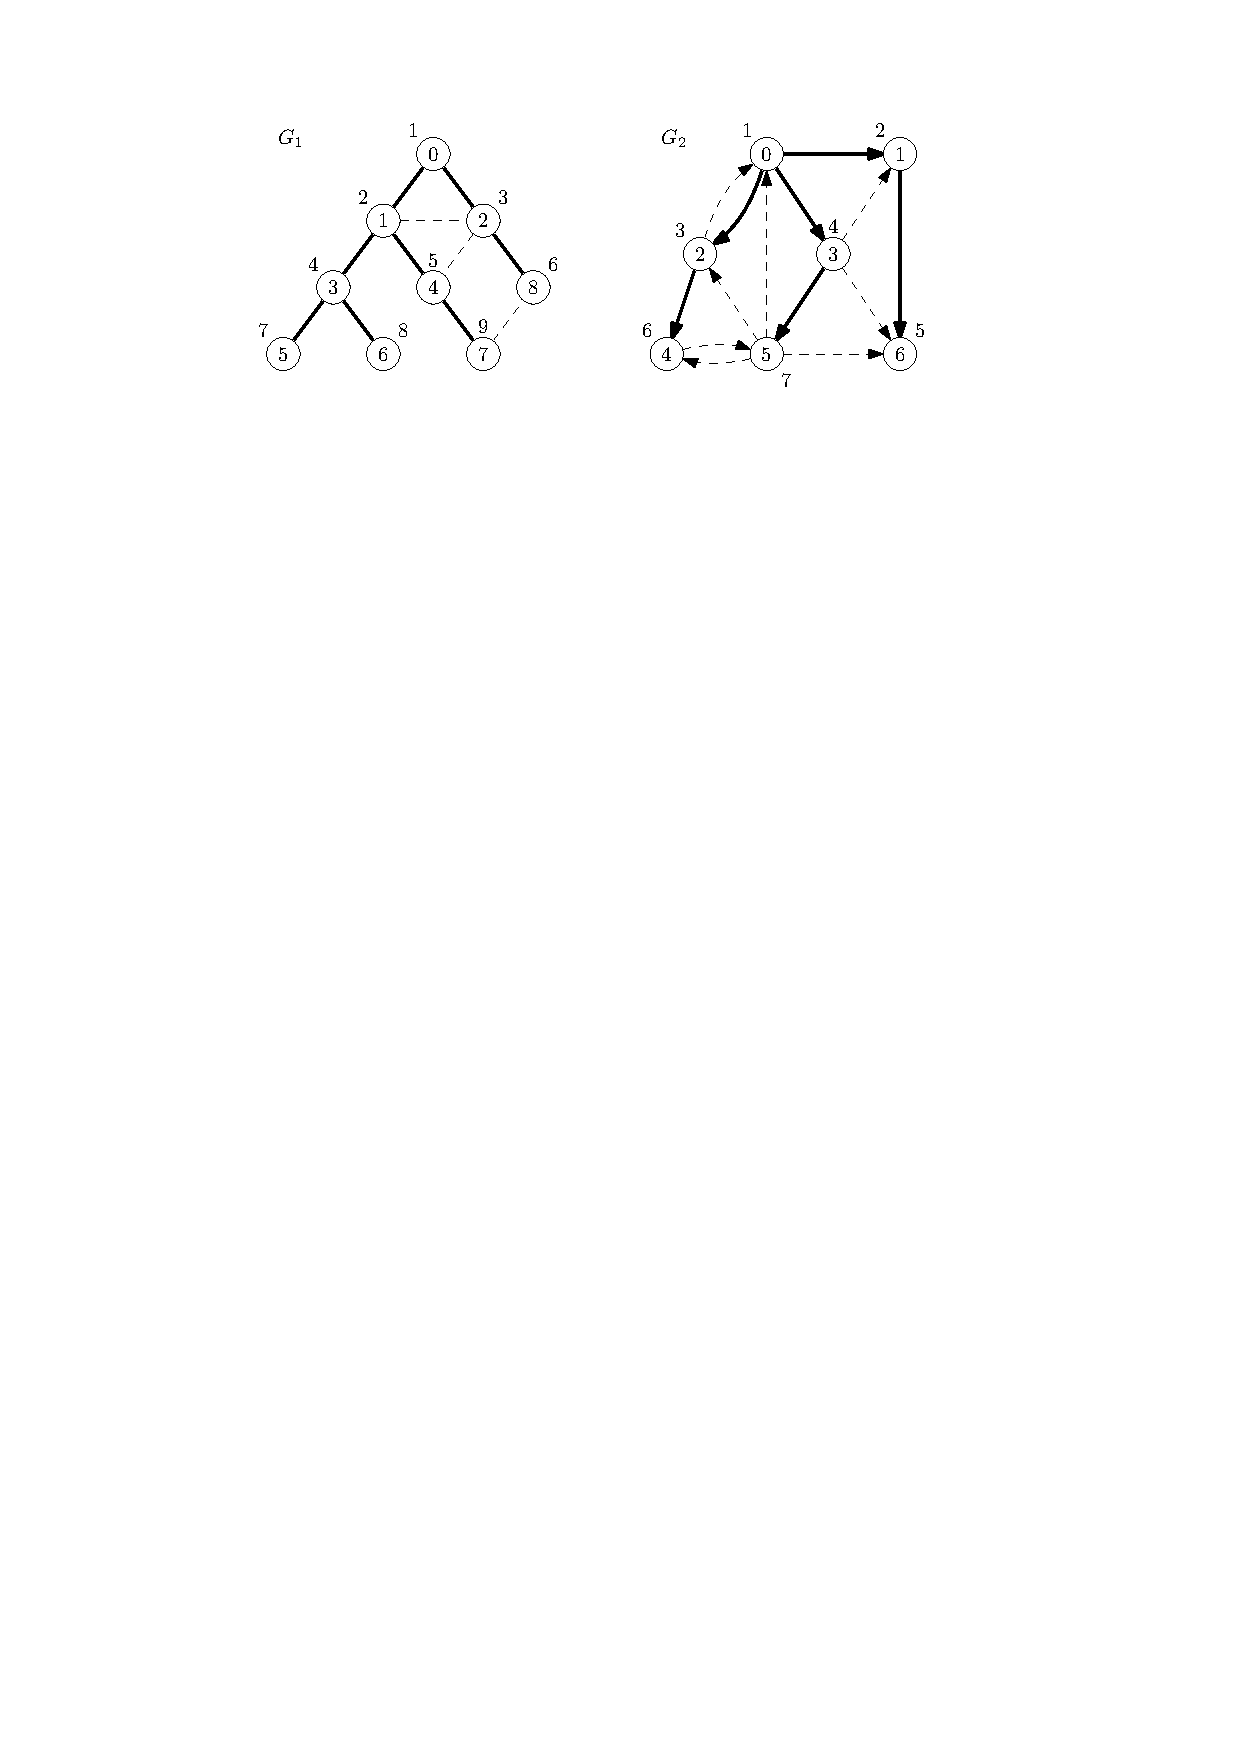
\includegraphics{graphEx2BFS}
	\caption{BFS trees for $G_1$ and $G_2$ of \cref{fig:graphExample2}, rooted at $0$.}
	\label{fig:graphEx2-BFS}
\end{figure}

\begin{Example}
In \cref{fig:graphEx2-BFS} we show the breadth-first search trees based on a BFS traversal of $G_1$ and $G_2$ in \cref{fig:graphExample2} starting at node $0$ . The
dashed arcs indicate the original arcs that are not part of the BFS trees. The numbering next to the 
\end{Example}

\begin{Boxample}[2]
Find a tree arc, cross arc, forward arc and back arc for each of the search trees in \cref{fig:graphEx2-BFS} (or say if that type of arc does not exist for that traversal).
\end{Boxample}

\section{Additional properties of breadth-first search}
\label{sec:bfs}

The first-in first-out processing of the grey nodes in BFS is ideally
handled by a queue. The pseudocode for BFS is in \cref{alg:BFScode,alg:BFSvisitcode}.
The timestamps $\seen, \done$ of DFS are of less use here;
it is more useful to record the number of steps from the root in the
array $d$.


\begin{algorithm}[H]
  \caption{Breadth-first search algorithm.}
    \label{alg:BFScode}
\begin{algorithmic}[1]
\Function{BFS}{digraph $G$}
	\State queue $Q$  
	\State array $\colour[0..n-1], \pred[0..n-1], d[0..n-1]$
	\For{$u \in V(G)$} 
		\State $\colour[u] \gets $ WHITE; $\pred[u] \gets $ NULL
	\EndFor
	\For{$s \in V(G)$} 
		\If{$\colour[s] = $ WHITE } 
			\State \algfont{BFSvisit}$(s)$
		\EndIf
	\EndFor
	\State \Return{$\pred, d$}
\EndFunction
\end{algorithmic}
\end{algorithm}
\begin{algorithm}[H]
  \caption{Breadth-first search visit algorithm.}
     \label{alg:BFSvisitcode}
  \begin{algorithmic}[1]
\Function{BFSvisit}{node $s$}
	\State $\colour[s] \gets $ GREY; $d[s] \gets 0$ 
	\State $Q$.\algfont{insert}$(s)$
	\While{\textbf{not} $Q$.\algfont{isEmpty}$()$}
		\State $u \gets Q$.\algfont{peek}$()$
		\For{each $v$ adjacent to $u$}
			\If{$\colour[v] = $ WHITE}
				\State $\colour[v] \gets $ GREY; $\pred[v] \gets u$; $d[v] \gets d[u]+1$
				\State $Q$.\algfont{insert}$(v)$
			\EndIf
		\EndFor
		\State $Q$.\algfont{delete}()
		\State $\colour[u] \gets $ BLACK
	\EndWhile
\EndFunction
\end{algorithmic}
\end{algorithm}

%A similar analysis to what we did for DFS also holds for BFS: it is also
%a linear time traversal algorithm, because the next grey and white node 
%can again be chosen in constant time.

It is rather obvious that BFS processes all nodes at distance 1, then
all nodes at distance 2, etc, from the root. The formal theorem stating this is given below without proof (see book for a simple inductive proof).

\begin{Theorem}
\label{thm:BFSdist}
Suppose we run \algfont{BFS} on a digraph $G$.
Let $v\in V(G)$, and let $r$ be the root of the search tree containing $v$. 
Then $d[v] = d(r, v)$.
\end{Theorem}

%\begin{proof}
%Note that since $d[v]$ is the length of a path of tree arcs
%from $r$ to $v$, we have $d[v] \geq d(r, v)$. We prove the result by
%induction on the distance. Denote the BFS search forest by $F$ and let $s$
%be the root of a tree in $F$. Then $d[s] = 0 = d(s, s)$ so the result is
%true for distance zero. Suppose it is true for all $v$ for which $d(s,
%v) < k$ and consider a node $v$ such that $d(s, v) = k \geq 1$. Choose
%a shortest path from $s$ to $v$ in $G$ and let $u$ be the penultimate
%node in the path. Then $d(s, u) = k - 1$ (it cannot be less, or it would
%contradict $d(s, v) = k$; on the other hand the subpath from $s$ to $u$
%must be a shortest path from $s$ to $u$, otherwise we could find a shorter
%one from $s$ to $v$). By the inductive hypothesis, $d[u] = d(s, u) = k -
%1$. Now $v$ must be seen after $u$ (otherwise $d[v] < k$, but we know
%$d[v] \geq d(s, v) = k$). Thus $v$ is seen in the loop through white
%neighbours of $u$, and so $d[v] = d[u] + 1 = k$. 
%\end{proof}

We can classify arcs, but the answer is not as nice as with DFS.

\begin{Theorem}
\label{thm:BFS-arcclass}
Suppose that we are performing \algfont{BFS} on a digraph $G$. Let $(v,
w)\in E(G)$ and suppose that we have just chosen the grey node $v$. 
Then
\begin{itemize}
\item
if $(v, w)$ is a tree arc then $\colour[w] = $ WHITE, $d[w] = d[v] + 1$
\item
if $(v, w)$ is a back arc, then $\colour[w] = $ BLACK, $d[w] \leq d[v] - 1$  
\item
There are no forward arcs.
\item
if $(v, w)$ is a cross arc then one of the following holds:
\begin{itemize}
\item $d[w] < d[v] - 1$, and $\colour[w] = $ BLACK;
\item $d[w] = d[v]$, and $\colour[w] = $ GREY;
\item $d[w] = d[v]$, and $\colour[w] = $ BLACK;
\item $d[w] = d[v] - 1$, and $\colour[w] = $ GREY;
\item $d[w] = d[v] - 1$, and $\colour[w] = $ BLACK.
\end{itemize}
\end{itemize}
\end{Theorem}

%\begin{proof}
%The arc is added to the tree if and only if $w$ is white. If the arc is
%a back arc, then $w$ is an ancestor of $v$; the FIFO queue structure
%means $w$ is black before the adjacency list of $v$ is scanned. 
%
%Now suppose that $(x, u)$ is a forward arc. Then since $u$ is a
%descendant of $x$ but not a child in the search forest, 
%Theorem~\ref{thm:BFSdist} yields $d[u]
%\geq d[x] + 2$. But by the last theorem we have $d[u] = d(s, u) \leq
%d(s, x) + 1 = d[x] + 1$, a contradiction. Hence no such arc exists.
%
%A cross arc may join two nodes on the same level, jump up one level,
%or jump up more than one level. In the last case, $w$ is already black
%before $v$ is seen. In the second case, $w$ may be seen before $v$,
%in which case it is black before $v$ is seen (recall $w$ is not the
%parent of $v$), or it may be seen after $v$, in which case it is grey
%when $(v, w)$ is explored. In the first case, $w$ may be seen before $v$ (in
%which case it is black before $v$ is seen), or $w$ may be seen after $v$
%(in which case it is grey when $(v, w)$ is explored).
%\end{proof}

In the special case of graphs we can say more.

\begin{Theorem}
\label{thm:BFS-grapharcclass}
Suppose that we have performed \algfont{BFS} on a graph $G$. Let $\{v,
w\}\in E(G)$. Then exactly one of the following conditions holds.

\begin{itemize}
\item
$\{v, w\}$ is a tree edge, $| d[w] - d[v] |= 1$;
\item
$\{v, w\}$ is a cross edge, $d[w] = d[v]$;
\item
$\{v, w\}$ is a cross edge, $| d[w] - d[v] | = 1$.
\end{itemize}
\end{Theorem}

%\begin{proof} By Theorem~\ref{thm:BFS-arcclass} there can be no forward
%edges, hence no back edges. A cross edge may not jump up more than
%one level, else it would also jump down more than one level, which is
%impossible by Theorem~\ref{thm:BFSdist}.
%\end{proof}

For a given BFS tree, we can uniquely label the vertices of
a digraph based on the time they were first seen. For the graph
$G_1$ of \cref{fig:graphExample2}, we label vertex 0 with 1,
vertices \set{1,2} with labels \set{2,3}, vertices \set{3,4,8} with
labels \set{4,5,6}, and the last vertex level \set{5,6,7} with labels
\set{7,8,9}. These are indicated in \cref{fig:graphEx2-BFS}.

\subsection*{Exercises}

\begin{Exercise}
\label{ex:doBFS}
Carry out \algfont{BFS} on the digraph with adjacency list given below. 
Show the state of the queue after each change in its state.
\newline
$$
\lightgraybox{
	\begin{tabular}{c|cccc}
		0 & 2 &   &   \\
		1 & 0 &   &   \\
		2 & 0 & 1 &   \\
		3 & 4 & 5 & 6 \\
		4 & 5 &   &   \\
		5 & 3 & 4 & 6 \\
		6 & 1 & 2 &   \\
	\end{tabular}
}
$$
\end{Exercise}


\begin{Exercise}
\label{ex:BFS-back-vs-cross}
How can we distinguish between a back and a cross arc while 
\algfont{BFS} is running on a digraph?

\end{Exercise}

\begin{Exercise}
\label{ex:BFS-cycle}
Explain how to determine whether the root of a BFS tree is contained in
a cycle, while the algorithm is running. You should find a cycle of
minimum length if it exists.
\end{Exercise}

\section{Priority-first search}
\label{sec:PFS}

Priority-first search is a more general and sophisticated form of traversal that encompasses both BFS and DFS (and others). 

\begin{itemize}
\item each grey node has associated with it an
integer \defnfont{key}. 
\item The interpretation of the key is of a priority: the
smaller the key, the higher the priority. 
\item The rule for choosing a new
grey node is to choose one with the smallest key.  
\item The key can either be assigned once when the node is first seen and then left unchanged, or could be updated at other times. We concentrate on unchanging keys here.
\item To mimic BFS, set the key for the node $v$ to be the time that $v$ turns grey. It will always remain as the lowest key until it turns black.
\item To mimic DFS, set the key for node $v$ to be $-\seen[v]$, so that the most recently seen node has the lowest key
\item The running time of PFS depends on how long it takes to find the minimum key value.
\item The rules described here implemented using an array take $\Omega(n)$ to find the lowest key so the algorithm is $\Theta(n^2)$. Contrast with with $\Theta(m+n)$ for standard traversal.
\item PFS is best described via the priority
queue ADT which has more efficient implementations than using a standard array.
\end{itemize}


%In the simplest form of PFS, the key value is assigned when the node
%becomes grey, and never updated subsequently. More generally, the key
%may be further updated at other times. We shall see both types in this
%book. The second type of PFS is used in optimization problems as we
%shall discuss in Chapter~\ref{ch:weighted}. 
%
%The first type of PFS includes both BFS and DFS. In BFS, the key
%value of $v$ can be taken as the time $v$ was first coloured grey.
%Note that this means that a given grey node can be selected many
%times---until it becomes black, in fact, it will always have minimum
%key among the grey nodes. By contrast, in DFS we can take the key
%value to be $-\seen[v]$. Then the last node seen always has minimum
%key. It cannot be chosen again until the nodes seen after it have
%become black.
%
%The running time of PFS depends mostly on how long it takes to find the
%minimum key value, and how long it takes to update the key values.
%
%In the array implementation mentioned above, finding the minimum key
%value takes time of order $n$ at each step, so the quantity $a$ is
%$\Omega(n)$. Thus a PFS of this type will take time in $\Omega(n^2)$.
%This is worse than the $\Theta(n+m)$ we obtain with BFS and DFS using
%adjacency lists and a queue or stack respectively. One reason is that a
%simple array is not a particularly good data structure for finding the
%minimum key. You have already seen a better one in Part I of this 
%book---the binary heap. In fact PFS is best described via the priority
%queue ADT (see Section~\ref{sec:app:adt-informal}).

Pseudocode demonstrating the PFS is presented in
\cref{fig:PFScode}. The subroutine \algfont{setKey} there is the
rule for giving the key value when a node is inserted. We do not include
any code for \algfont{setKey}.

\begin{algorithm}[H]
  \caption{Priority-first search algorithm (first kind)}
  \label{fig:PFScode}
\begin{algorithmic}[1]
\Function{PFS}{digraph $G$}
	\State priority queue $Q$  
	\State array $\colour[0..n-1], \pred[0..n-1]$
	\For{$u \in V(G)$} 
		\State $\colour[u] \gets $ WHITE; $\pred[u] \gets $ NULL
	\EndFor
	
	\For{$s \in V(G)$} 
		\If{$\colour[s] = $ WHITE } 
			\State \algfont{PFSvisit}$(s)$
		\EndIf
	\EndFor
	\State \Return{$\pred$}
\EndFunction
\Function{PFSvisit}{node $s$}
	\State $\colour[s] \gets $ GREY 
	\State $Q$.\algfont{insert}($s$, \algfont{setKey}$(s)$)
	\While{\textbf{not} $Q$.\algfont{isEmpty}$()$}
		\State $u \gets Q$.\algfont{peek}$()$
		\If{$u$ has a neighbour $v$ with $\colour[v] = $ WHITE}
			\State $\colour[v] \gets $ GREY
			\State $Q$.\algfont{insert}$(v$, \algfont{setKey} $(v))$
		\Else
			\State $Q$.\algfont{delete}
			\State $\colour[u] \gets$ BLACK
		\EndIf
	\EndWhile
\EndFunction
\end{algorithmic}
\end{algorithm}


%\subsection*{Exercises}
\chapter{Cycles, Girth and Topological Sort}


\section{Acyclic digraphs and topological ordering}
\label{sec:dag}

In this section we show how to arrange, when possible, the nodes
of a digraph into a topological or precedence order.  Many computer
science applications require us to find precedences (or dependencies)
among events, such as a compiler evaluating sub-expressions of an
expression like that shown in \cref{fig:prec}.

\begin{figure}[hbtp]
	\centering
	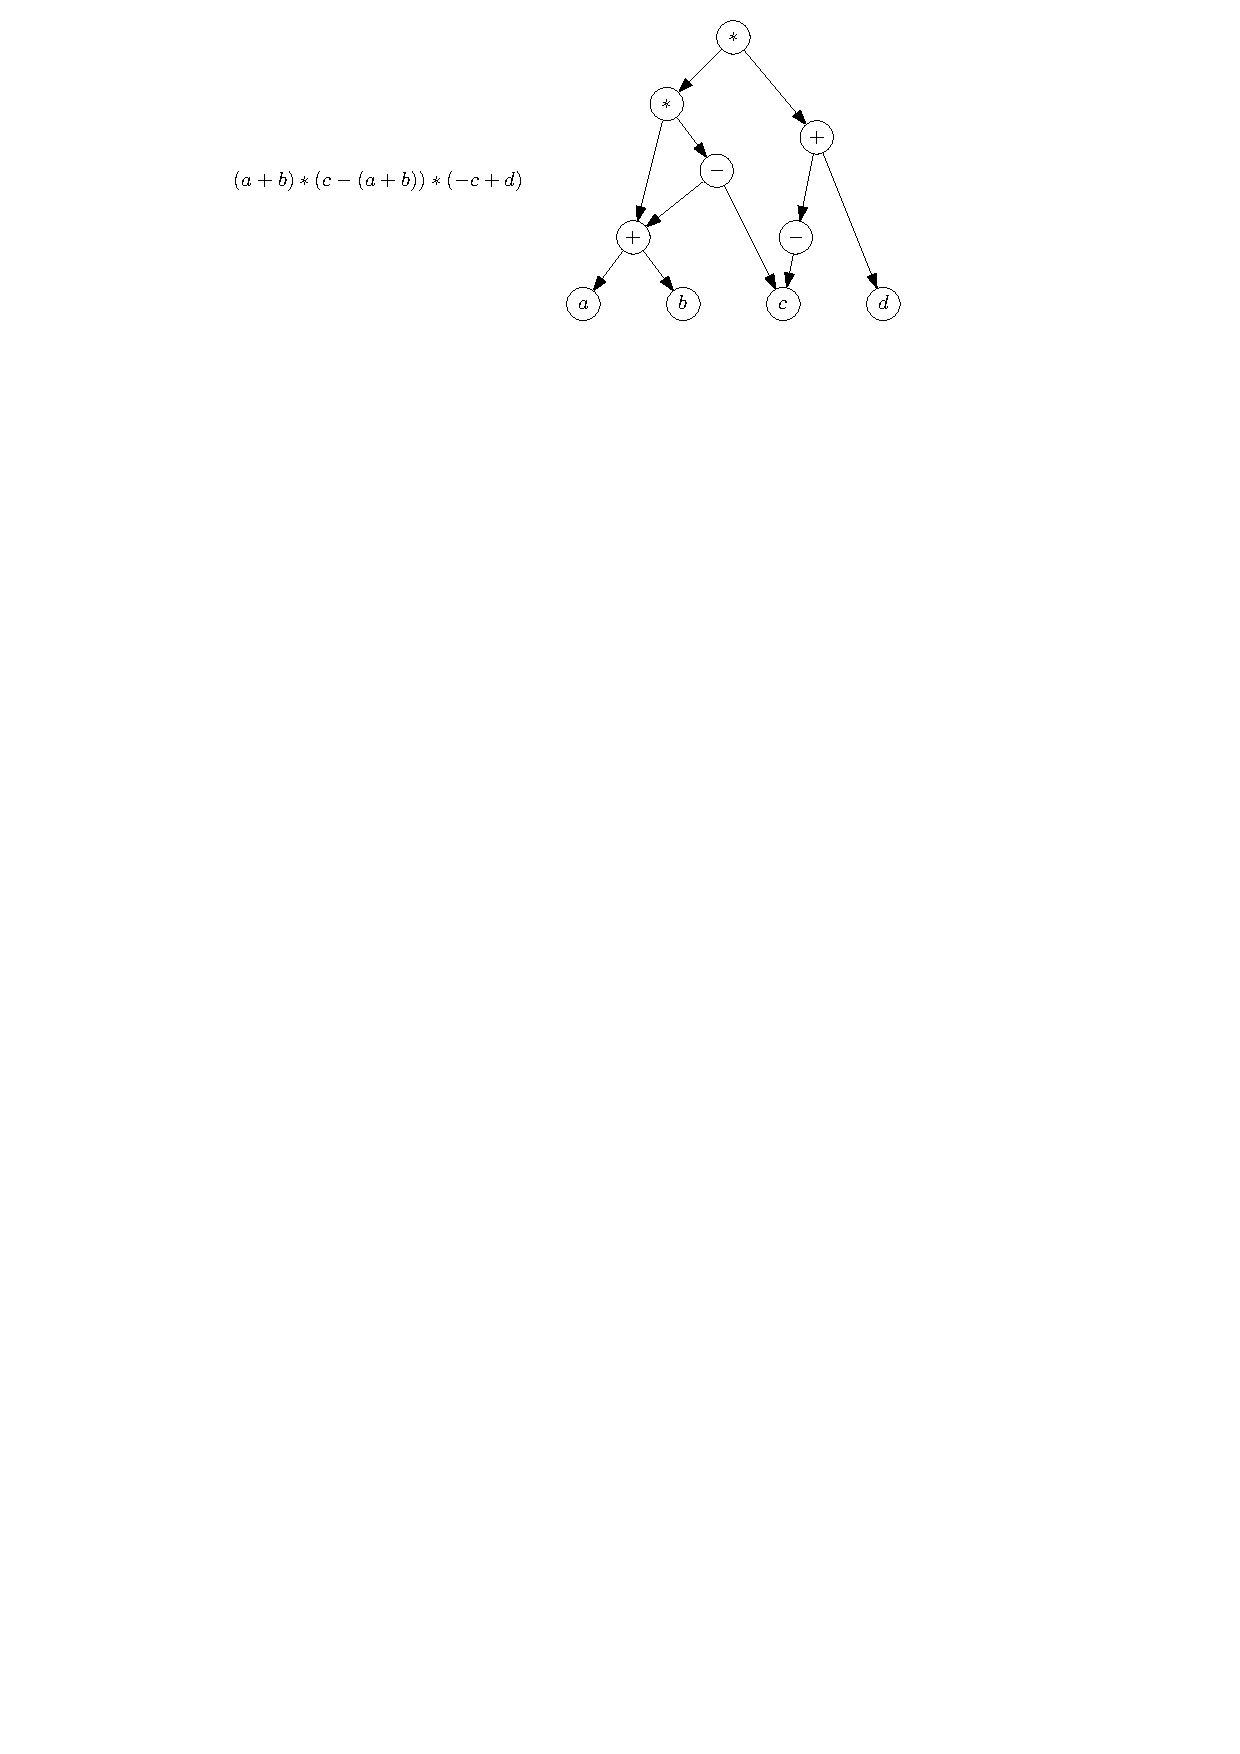
\includegraphics{precedence}
	\caption{Digraph describing structure of an arithmetic expression.}
	\label{fig:prec}
\end{figure} 

Here the compiler would need to compute, for example, both $(a+b)$ and
$c$ before it can compute $c-(a+b)$.

\begin{Definition}
Let $G$ be a digraph. A \defnfont{topological sort} of $G$ is a linear
ordering of all its vertices such that if $G$ contains an arc $(u,v)$,
then $u$ appears before $v$ in the ordering.
\end{Definition}

The term topological sort comes from the study of partial orders and is
sometimes called a \defnfont{topological order} or \defnfont{linear order}.
 If a topological sort exists, then it is possible to draw a picture  of
$G$ with all nodes in a straight line, and the arcs ``pointing the same
way".

A digraph without cycles is commonly called a \defnfont{DAG}, an
abbreviation for \textbf{d}irected \textbf{a}cyclic
\textbf{g}raph. It is much easier for a digraph to be a
DAG than for its underlying graph to be acyclic. % (see Exercise~\ref{}). 

For our arithmetic expression example above, a linear
order of the sub-expression DAG gives us an order (actually the reverse
of the order) where we can safely evaluate the expression.

Clearly if the digraph contains a cycle, it is not possible to find
such a linear ordering. This corresponds to inconsistencies in the
precedences given, and no scheduling of the tasks is possible.

\begin{Example}
\label{eg:toporder}
In \cref{fig:toporder} we list three DAGs and possible topological
orders for each. Note that adding more arcs to a DAG  reduces the number
of topological orders it has.  This is because each arc $(u,v)$ forces
$u$ to occur before $v$, which restricts the number of valid permutations
of the vertices.
\end{Example}

\begin{Boxample}[1]
A graph with all possible topological orders and drawn with topological order $0, 1, 2, 3, 4$.  Draw the graph for topological order $0, 2, 1, 4, 3$. 
\begin{center}
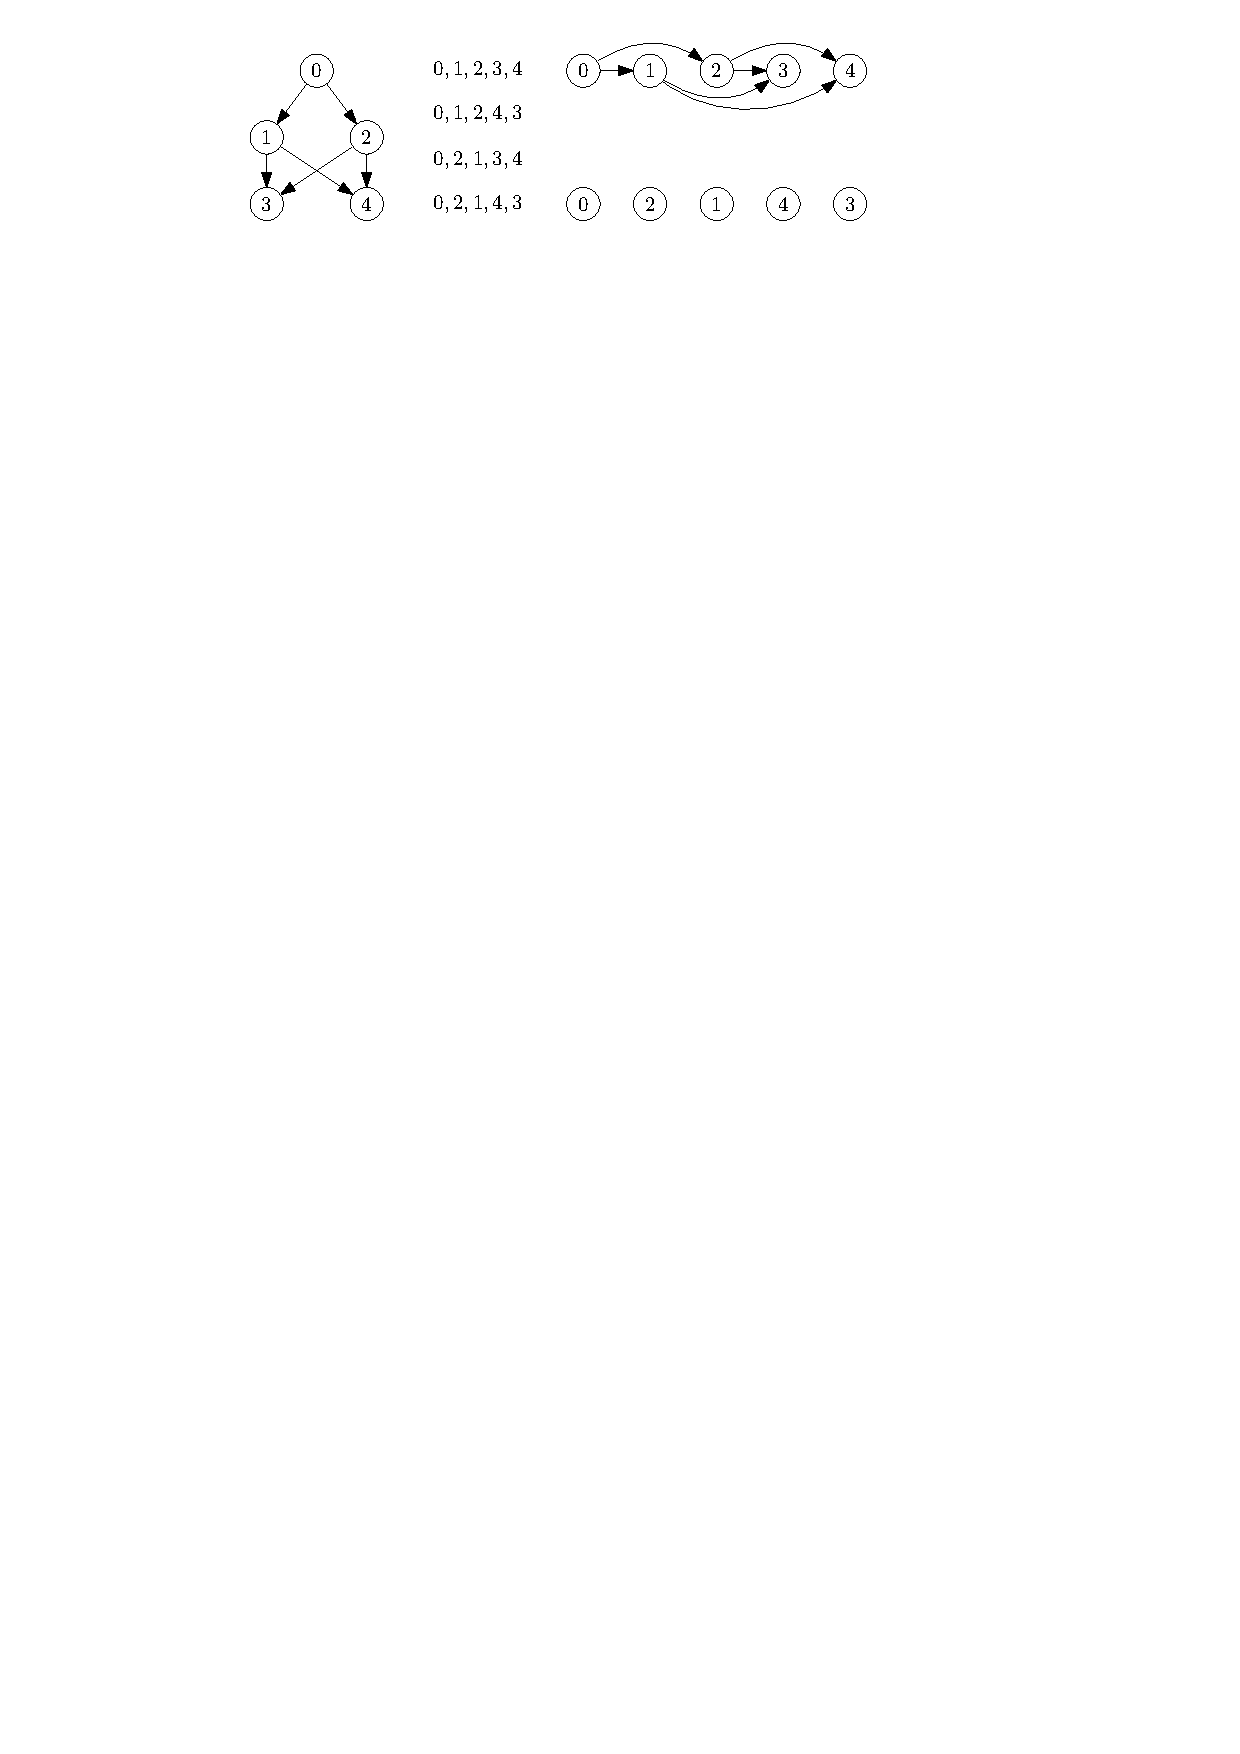
\includegraphics{topologicalOrder1}
\end{center}
Find a topological order of the following graph and draw it.
\begin{center}
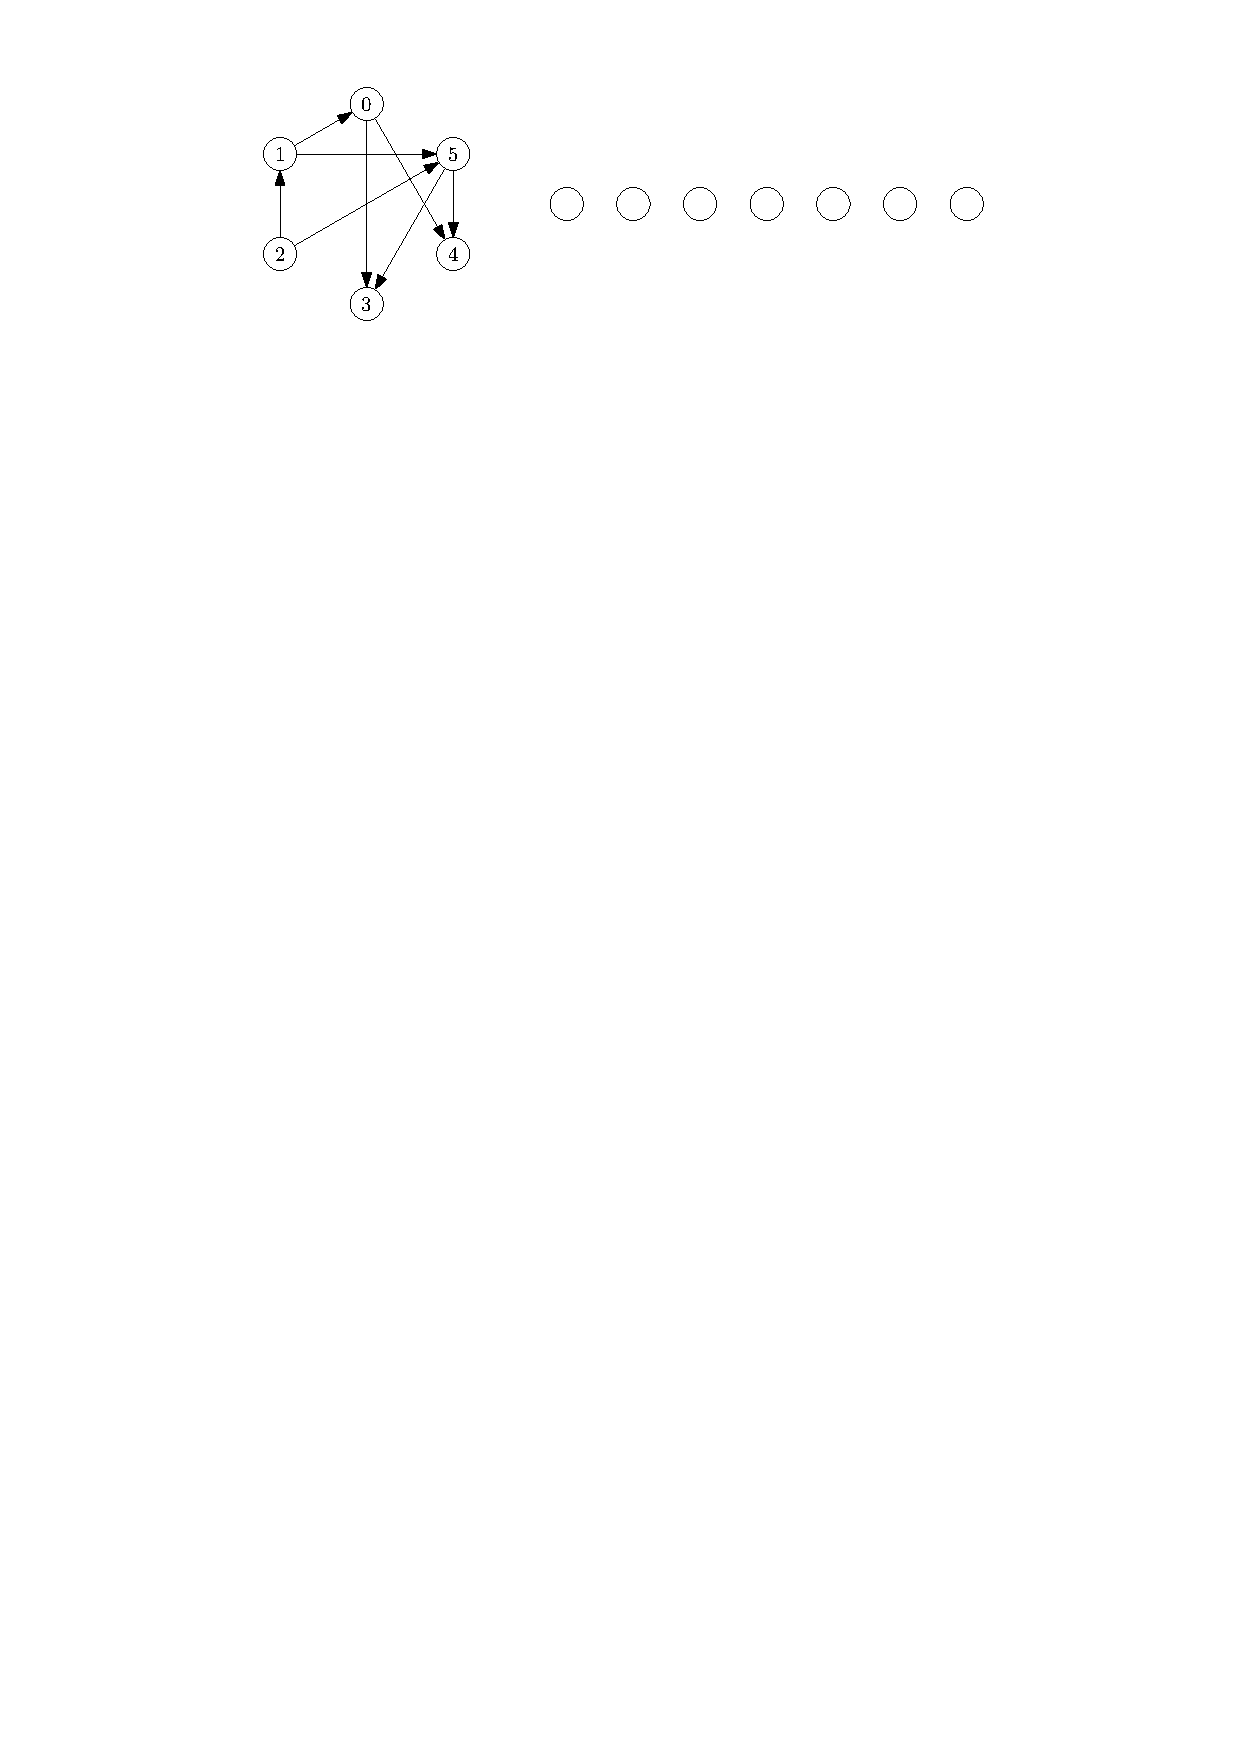
\includegraphics{topologicalOrder2}
\end{center}
List all possible topological orders of the following graph.
\begin{center}
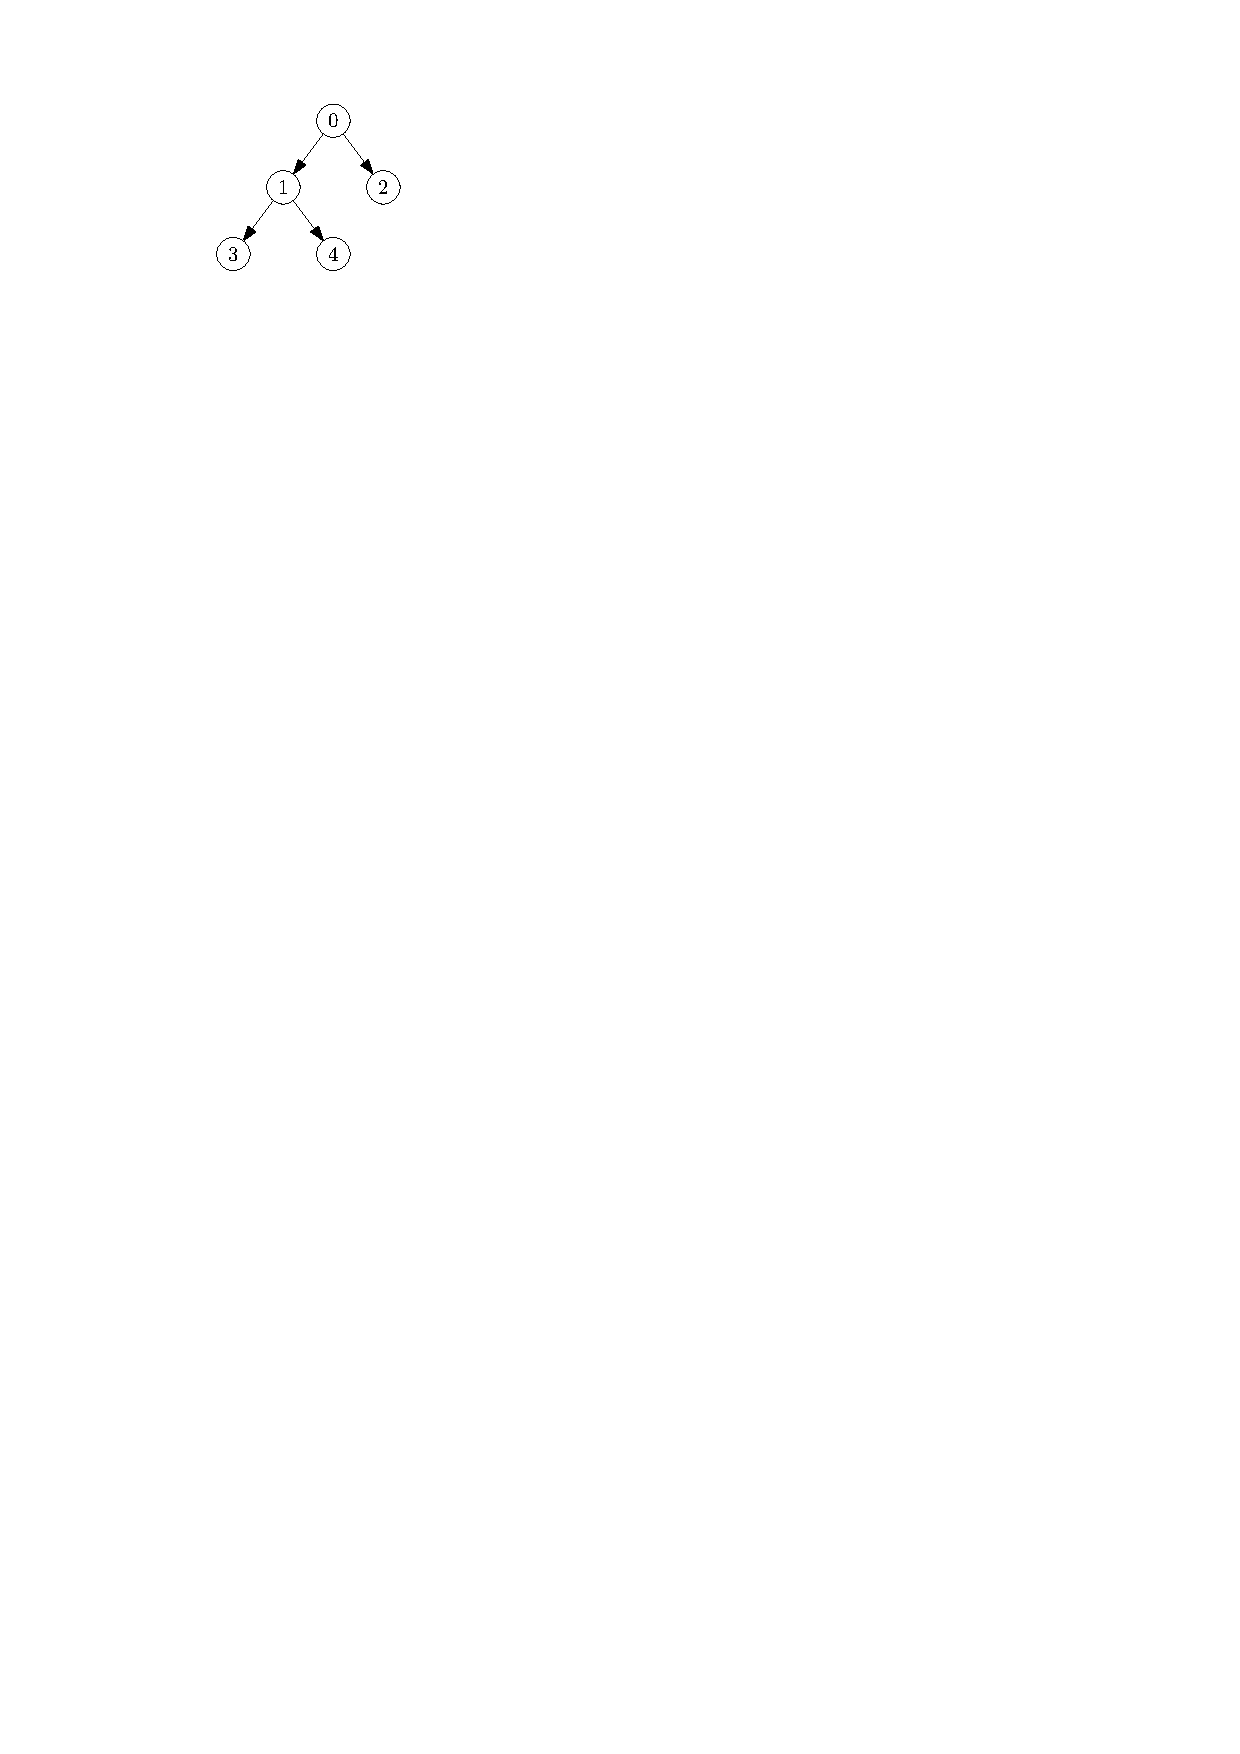
\includegraphics{topologicalOrder3}
\end{center}
\end{Boxample}
% \begin{figure}
% \centerline{\IpeScale{80}\Ipe{./figs/graphEx4.ipe}}
% \caption{Topological orders of some DAGs.}
% \label{fig:toporder}
% \end{figure}

The algorithms for computing \boldfont{all} topological orders are
more advanced than what we have time or space for here. We show how to
compute one such order, however.

First we note that \boldfont{if} a topological sort of a DAG $G$
is possible, then there must be a source node in $G$. The source
node can be first in a topological order, and no node that is not
a source can be first (because it has an in-neighbour that must
precede it in the topological order). 

%\newpage

\begin{Theorem}
\label{thm:topDAG}
A digraph has a topological order if and only if it is a DAG.
\end{Theorem}

\begin{proof} 
First show that every DAG has a source (see
exercise~\ref{ex:DAG-sink}).  Given this, we proceed as follows. Deleting
a source node creates a digraph that is still a DAG, because deleting
a node and some arcs cannot create a cycle where there was none
previously. Repeatedly doing this gives a topological order.
\end{proof}

This theorem then gives an algorithm (\defnfont{zero-indegree sorting})
for topologically sorting a DAG $G$.

So far we have not shown how to determine whether a given digraph is
a DAG. But if we apply zero-indegree sorting to a digraph that is not
a DAG, eventually it will stop because no source node can be found at
some point (otherwise we would obtain a topological order and hence the
digraph would be a DAG).

There is another way to determine acyclicity and topologically sort a
DAG, based on DFS. If $G$ contains a cycle,  DFS must eventually reach
a node that points to one that has been seen before. In other words, we
will detect a back arc. The details and proof that this works now follow.

\begin{Theorem}
\label{thm:findDAG}
Suppose that DFS is run on a digraph $G$. Then $G$ is acyclic if and
only if there are no back arcs.
\end{Theorem}

\begin{proof}
Suppose that we run DFS on $G$. Note that if there is a
back arc $(v, u)$, then $u$ and $v$ belong to the same tree $T$, with
root $s$ say. Then there is a path from $s$ to $u$, and there is a path
from $u$ to $v$ by definition of back arc. Adding the arc $(v, u)$ gives
a cycle. 

Conversely, if there is a cycle $v_0\, v_1\, \dots \, v_n\, v_0$, we may
suppose without loss of generality that $v_0$ is the first node of the
cycle  visited by the DFS algorithm. We claim that $(v_n, v_0)$ is a
back arc. To see why this is true, first note that during the DFS $v_0$ is 
linked to $v_n$ via a path of unvisited nodes (possibly of length shorter 
than $n$).  We have $v_n$ as a descendant of $v_0$ in the DFS tree and
a back arc ($v_n, v_0$).
\end{proof}

One valid topological order is simply the reverse of the DFS finishing times.

\begin{Theorem}
Let $G$ be a DAG. Then listing the nodes in reverse order of DFS
finishing times yields a topological order of $G$.
\end{Theorem}

\begin{proof} 
Consider any arc $(u,v)\in E(G)$. Since $G$ is a DAG,
the arc is not a back arc by Theorem~\ref{thm:findDAG}. In the other three
cases, Exercise~\ref{ex:DFS-arc-class} shows that $\done[u] > \done[v]$,
which means $u$ comes before $v$ in the alleged topological order.
\end{proof}

We can therefore just run DFS on $G$, and stop if we find a back
arc. Otherwise printing the nodes in reverse order of finishing time
gives a topological order. Note that printing the nodes in order of
finishing time gives a topological order of the reverse digraph $G_r$.

%\subsection*{Exercises}
%
%\begin{Exercise}
%\label{ex:DAG-vs-tree}
%Give an example of a DAG whose underlying graph contains a cycle. Make
%your example as small as possible.
%\end{Exercise}
%
%\begin{Exercise}
%\label{ex:DAG-sink}
%Prove that every DAG must have at least one source and at least one sink.
%\end{Exercise}
%
%\begin{Exercise}
%\label{ex:sillytopsort}
%Show that the following method for topologically sorting a DAG does not work in 
%general: print the nodes in order of visiting time.
%\end{Exercise}
%
%\begin{Exercise} 
%\label{ex:profP}
%Professor P has the following information taped to his mirror, to help
%him to get dressed in the morning.
%
%Socks before shoes; underwear before trousers; trousers before belt;
%trousers before shoes; shirt before glasses; shirt before tie; tie
%before jacket; shirt before hat; shirt before belt.
%
%Find an acceptable order of dressing for Professor P.
%\end{Exercise}
%
%\begin{Exercise}
%\label{ex:zero-indeg-runtime}
%What is the time complexity of zero-indegree sorting? 
%\end{Exercise}
%
%
%\begin{Exercise}
%\label{ex:forest}
%Let $G$ be a graph. There is an easy way to show that $G$ is acyclic.
%It is not hard to show (see Section~\ref{sec:app:trees}) that a graph $G$ is 
%acyclic if and only if $G$ is a forest, that is, a union of (free) trees.
%
%Give a simple way to check whether a graph $G$ is acyclic. Does the method 
%for finding a DAG given above work for acyclic graphs also?
%\end{Exercise}

\chapter{Connectivity, components, strong components}

\section{Connectivity}
\label{sec:connectivity}

For many purposes it is useful to know whether a digraph is ``all in one
piece", and if not, to decompose it into pieces. We now formalize these
notions. The situation for graphs is easier than that for digraphs.

\begin{Definition} 
A graph is \defnfont{connected} if for each pair of 
vertices $u, v\in V(G)$, there is a path between them.
\end{Definition}

In \cref{eg:graphExample} the graph $G_1$ is connected, as is the
underlying graph of $G_2$. 

If a graph is not connected, then it must have more than one ``piece".
More formally, we have the following.

\begin{Theorem}
\label{thm:components}
Let $G$ be a graph. Then $G$ can be uniquely written as a union of
subgraphs $G_i$ with the following properties:
\begin{itemize}
\item each $G_i$ is connected
\item if $i\neq j$, there are no edges from any vertices in $G_i$ 
to any vertices in $G_j$
\end{itemize}
\end{Theorem}

\begin{proof}
Consider the relation $\sim$ defined on $V(G)$, given by $u\sim v$ if
and only if there is a path joining $u$ and $v$ (in other words, $u$ and
$v$ are each reachable from the other). Then $\sim$ is an equivalence
relation and so induces a partition of $V(G)$ into disjoint subsets. The
subgraphs $G_i$ induced by these subsets have no edges joining them by
definition of $\sim$, and each is connected by definition of $\sim$.
\end{proof}

The subgraphs $G_i$ above are called the \defnfont{connected components}
of the graph $G$. Clearly, a graph is connected if and only if it has
exactly one connected component.

\begin{Example}
\label{eg:components}
The graph obtained by deleting two edges from a triangle has 2 connected 
components.
\end{Example}

We can determine the connected components of a graph easily by using a
traversal algorithm. The following obvious theorem explains why.

\begin{Theorem}
\label{thm:trav-comps}
Let $G$ be a graph and suppose that DFS or BFS is run on $G$. Then the
connected components of $G$ are precisely the subgraphs spanned by the
trees in the search forest. 
\end{Theorem}

\begin{proof}
The result is true for any traversal procedure, as we have already observed in 
Theorem~\ref{thm:trav}. The trees of the search forest have no edges joining 
them, and together they span $G$.
\end{proof}

So we need only run BFS or DFS on the graph, and keep count
of the number of times we choose a root---this is the number of
components. We can store or print the vertices and edges in each
component as we explore them. Clearly, this gives a linear time algorithm
for determining the components of a graph.

So far it may seem that we have been too detailed in our treatment of 
connectedness. After all the above results are all rather obvious.
However, now consider the situation for digraphs. The intuition of ``being all 
in one piece" is not as useful here. In
\cref{eg:graphExample} the graph $G_1$ is connected, as is the
underlying graph of $G_2$. They are ``all in one piece", but not the
same from the point of view of reachability. For example, in digraph
$G_2$, node $2$ is a sink. This motivates the following definition.

\begin{Definition}
A digraph $G$ is \defnfont{strongly connected} if for each pair of nodes $u, v$ 
of $G$, there is a path in $G$ from $u$ to $v$.
\end{Definition}

\begin{note}
In other words, $u$ and $v$ are each reachable from the other.

\

Suppose that the underlying graph of $G$ is connected (some authors call
this being \defnfont{weakly connected}), but $G$ is not strongly
connected. Then if $G$ represents a road network, it is possible to get
from any place to any other one, but at least one such route will be
illegal: one must go the wrong way down a one-way street. 
\end{note}

A strongly connected digraph must contain many cycles: indeed, if $v$ and
$w$ are different nodes, then there is a path from $v$ to $w$ and a path
from $w$ to $v$, so $v$ and $w$ are contained in a cycle. Conversely, if
each pair of nodes is contained in a cycle, then the digraph is clearly
strongly connected.

Again, we can define \defnfont{strongly connected components} in a
way that is entirely analogous to component for graphs. The proof
above for connected components generalizes to this situation.

%\newpage
\begin{Theorem}
\label{thm:scc}
Let $G=(V, E)$ be a digraph. Then $V$ can be uniquely written as a union of
disjoint subsets $V_i$, with each corresponding induced subdigraph $G_i$ being
a strongly connected component of $G$.
\end{Theorem}

\begin{proof} Consider the relation $\sim$ defined on $V$, given by
$u\sim v$ if and only if there is a path joining $u$ and $v$ and a path
joining $v$ and $u$ (in other words, $u$ and $v$ are each reachable
from the other). Then $\sim$ is an equivalence relation and so induces
a partition of $V$ into disjoint subsets.  By definition, each 
subdigraph $G_i$ is strongly connected and of maximal order.
\end{proof}

\begin{Example}\label{eg:scc}
A digraph and its three (uniquely determined) strongly connected
components are displayed in \cref{fig:scc}. Note that there are
arcs of the digraph not included in the strongly connected components.
\end{Example}

\begin{figure}[htbp]
\centering
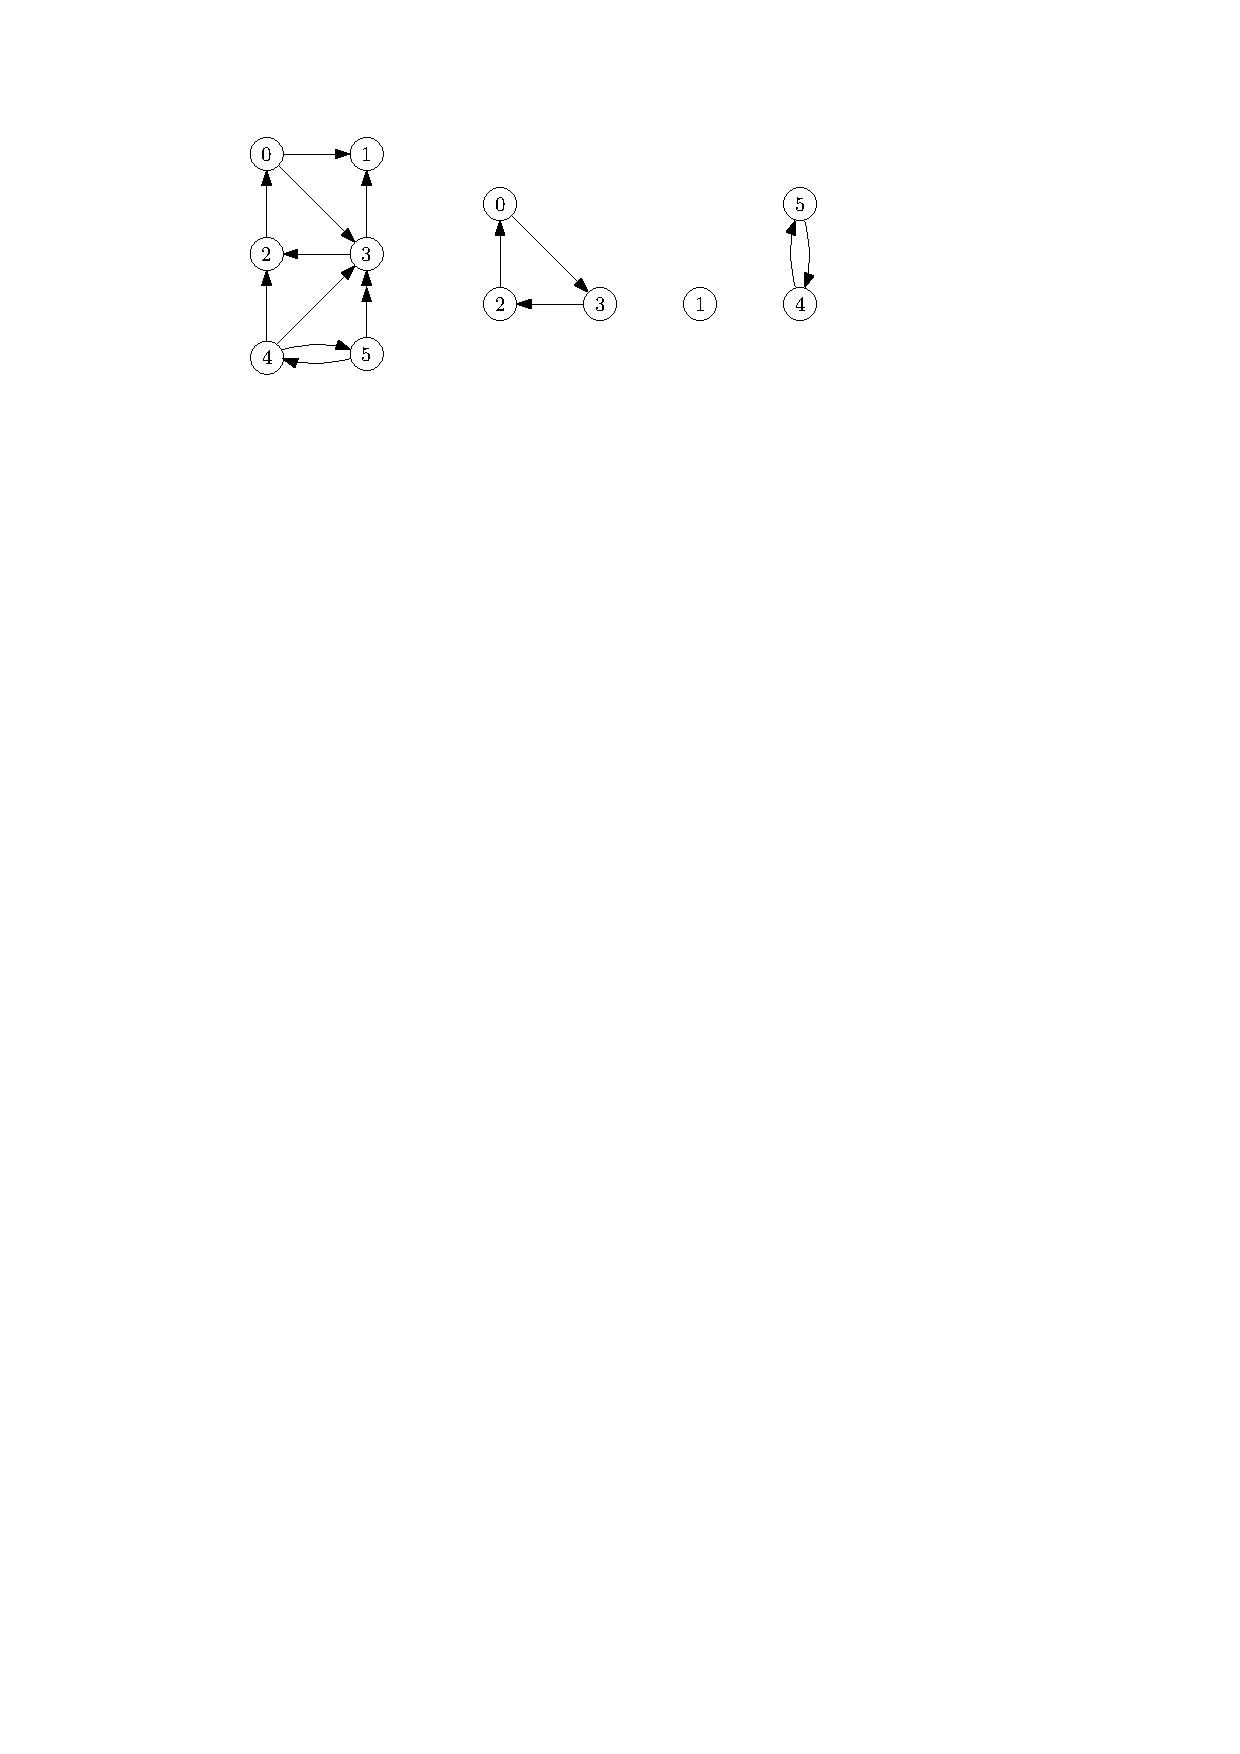
\includegraphics{SCC}
\caption{A digraph and its strongly connected components.}
\label{fig:scc}
\end{figure}

Note that if the underlying graph of $G$ is connected but $G$ is
not strongly connected, then  there are strong components $C_1$ and
$C_2$ such that it is possible to get from $C_1$ to $C_2$ but not
from $C_2$ to $C_1$. If $C_1$ and $C_2$ are different strong
components, then any arcs between them must either all point from
$C_1$ to $C_2$ or from $C_2$ to $C_1$.  Suppose that we imagine
each strong component shrunk to a single node (so we ignore the
internal structure of each component, but keep the arcs between
components). Then in the digraph resulting, if $v\neq w$ and we can
get from $v$ to $w$ then we cannot get from $w$ to $v$. In other
words, no pair of nodes can belong to a cycle, and hence the digraph
is acyclic. See \cref{fig:sccdecomp}. Note that the converse
is also true: if we have an acyclic digraph $G$ and replace each
node by a strongly connected digraph, the strongly connected
components of the resulting digraph are exactly those digraphs that
we inserted.

\begin{figure}[htbp]
\centering
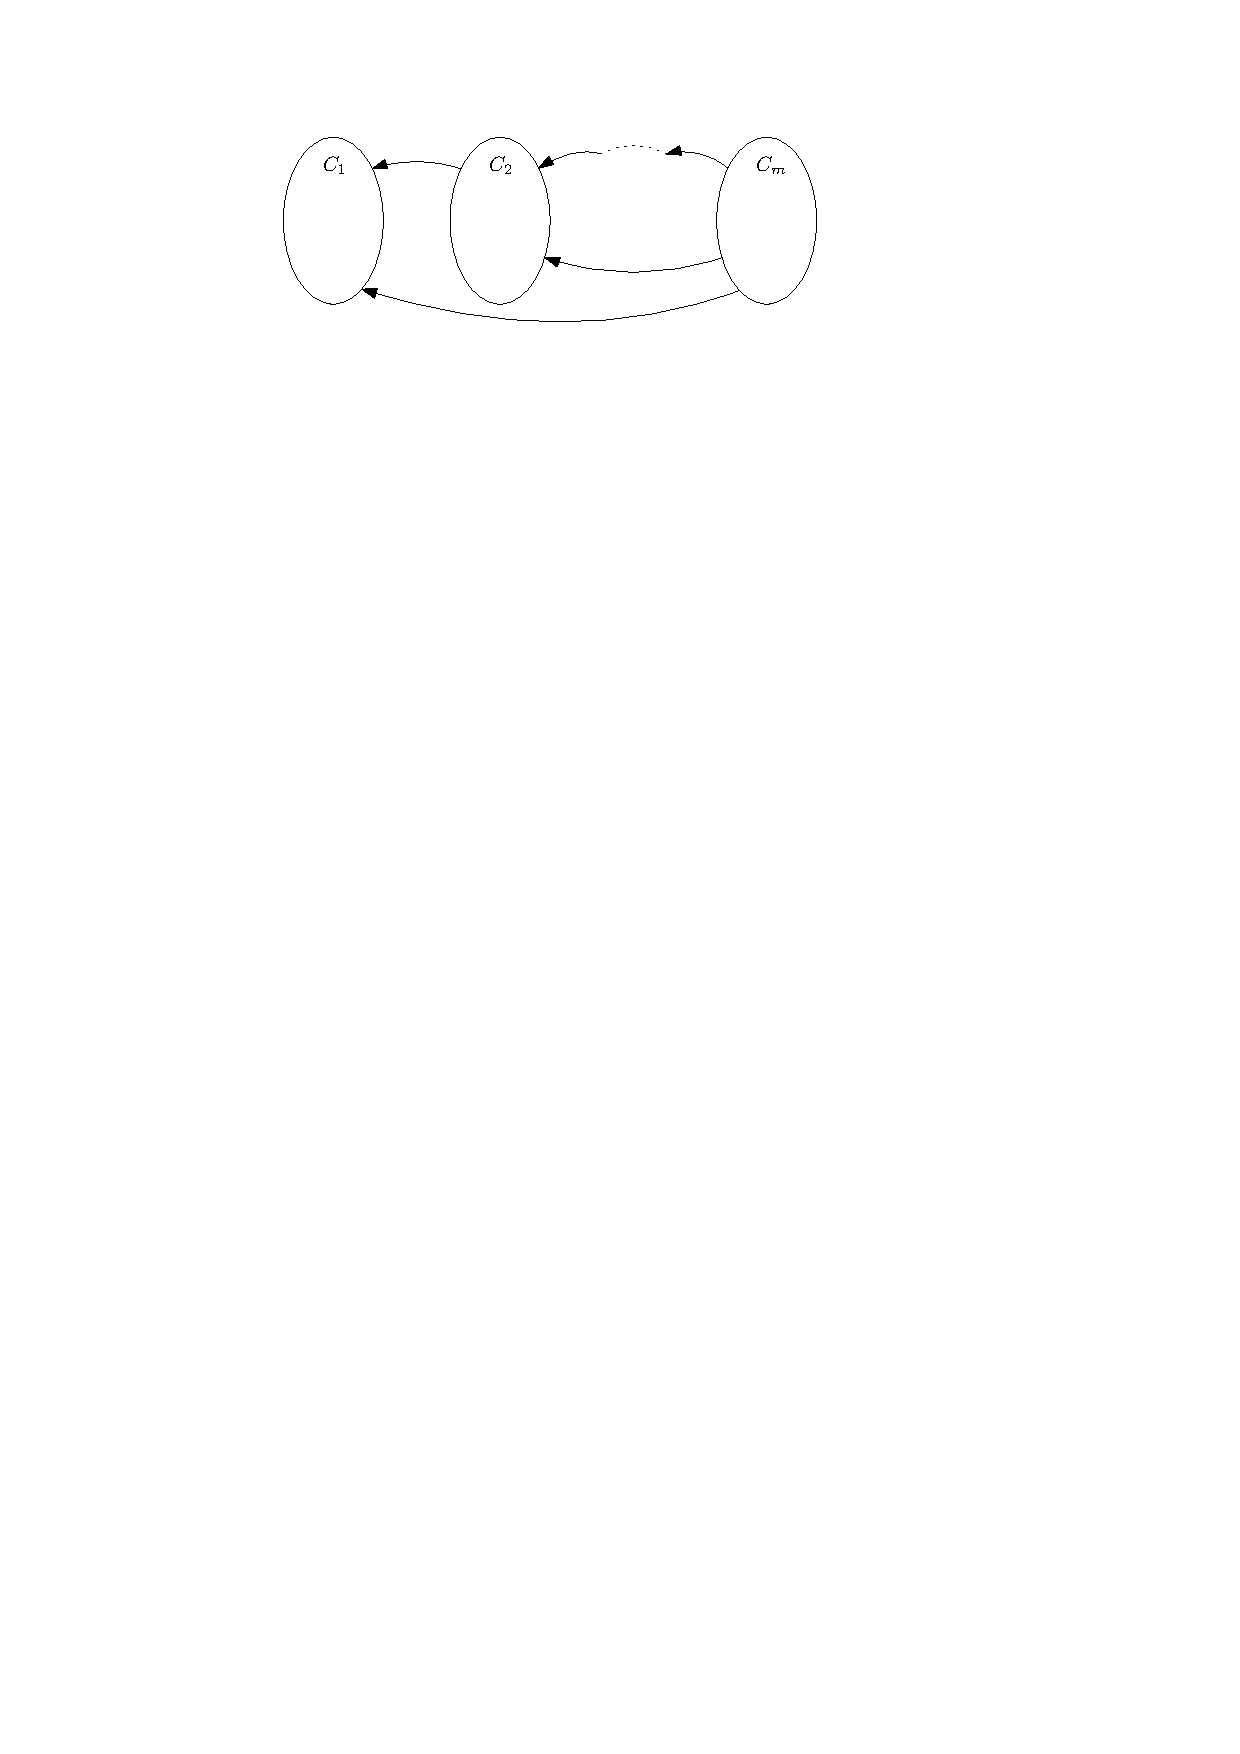
\includegraphics{decomposition2}
\caption{Structure of a digraph in terms of its strong components.}
\label{fig:sccdecomp}
\end{figure}

Note the similarity between this and the search forest decomposition
in \cref{fig:travdecomp}. In that case, if we shrink each
search tree to a point, the resulting digraph is also acyclic.

How to determine the strongly connected components? First we observe
that the previous method for graphs definitely fails (see
Exercise~\ref{ex:DFSfails}). To decide whether a digraph is strongly
connected we could run \algfont{BFSvisit} or \algfont{DFSvisit}
originating from each node in turn and see whether each of the $n$ trees
so generated spans the digraph. However the running time of such an
algorithm is $\Theta(n^2+nm)$.

We can do better by using DFS more cleverly. 

Consider the reverse $G_r$. The strong components of $G_r$ are the
same as those of $G$. Shrinking each strong component to a point,
we obtain  acyclic digraphs $H$ and $H_r$. Consider a sink $S_1$ in
$H_r$. If we run DFS on $G_r$ starting  in the strong component
$S_1$, we will reach every node in that component \boldfont{and no
other nodes of $G_r$}. The DFS tree will exactly span $S_1$. Now
choose the next root to lie in the strong component $S_2$ node of
$H_r$ whose only possible out-neighbour is $S_1$ (this is possible
by the same reasoning used for zero-indegree sort, except here we
deal with outdegree). The DFS will visit all of $S_2$ and no other
nodes of $G_r$ because all other possible nodes have already been
visited. Proceed in this way until we have visited all strong
components.

We have shown that if we can choose the roots correctly, then we can
find all strong components. Now of course we don't know these components
\boldfont{a priori}, so how do we identify the roots to choose?

Whenever there is a choice for the root of a new search tree, it must
correspond to a new node of the DAG $H_r$. We want at least a reverse
topological order of $H_r$. This is simply a topological order for
$H$. Note that in the case where $H=G$ (each strong component has just
one point), then $G$ is a DAG. The method above will work if and only
if we choose the roots so that each tree in the DFS for $G_r$ has only
one point. We just need a topological order for $G$, so run DFS on $G$
and print the nodes in reverse order of finishing time. Then choose the
roots for the DFS on $G_r$ in the printed order.

It therefore seems reasonable to begin with a DFS of $G$. Furthermore,
an obvious choice is: in the DFS of $G_r$, \boldfont{choose each new root
from among white nodes that finished latest in $F$}.

Then each DFS tree in the search of $G_r$ definitely contains the strong
component $S$ of the root $r$. To see this, note that no node in that
strong component could have been visited before in $G_r$, otherwise $r$
would have already been visited. By \cref{thm:white-path}, every
node in the strong component of $r$ is a descendant of $r$.

The only thing that could go wrong is that a search tree in $G_r$
might contain more than one strong component. This cannot happen,
as we now prove.

\begin{Theorem} \label{thm:scc-alg} 
If the following rule for choosing roots is used in the algorithm
described above, then each tree in the second search forest spans a
strong component of $G$, and all strong components arise this way.

Rule: use the white node whose finishing time in $F$ was largest.
\end{Theorem}

\begin{proof}
Suppose that a search tree in $G_r$ does  contain more than one strong
component. Let $S_1$ be the first strong component seen in $G_r$ and let
$S_2$ be another, and let the roots be $r, s$ respectively. Note that by
the rule for choosing nodes $r$ was the first node of $S_1$ seen in $F$
(by Theorem~\ref{thm:white-path}, every node of $S_1$ is a descendant
of the first one seen, which therefore has latest finishing time). The
analogous statement holds for $s$ and $S_2$.

By the rule for choosing roots, we have $\done[r] > \done[s]$ in $F$. We
cannot have $\seen[s] > \seen[r]$ in $F$, for then $s$ would be a descendant
of $r$ in $F$ and in $G_r$, so they would belong to the same strong
component. Thus $\seen[r] > \seen[s]$ in $F$. Hence $S_2$ was explored
in $F$ before $r$ (and hence any node of $S_1$) was seen. But then $r$
would have been reachable from $s$ in $G$ via a path of white nodes,
so Theorem~\ref{thm:white-path} shows that $r$ and $s$ are in the same
strong component, another contradiction.
\end{proof} 

The above algorithm runs in linear time with adjacency lists, since each
DFS and the creation of the reverse digraph take linear time. We only
need to remember  while performing the first DFS to store the nodes in
an array in order of finishing time. 

\subsection*{Exercises}

\begin{Exercise}
\label{ex:DFSfails}
Give an example to show that a single use of DFS does not in general
find the strongly connected components of a digraph.
\end{Exercise}

\begin{Exercise}
\label{ex:dolinscc}
Carry out the above  algorithm by hand on the digraph of
\cref{eg:scc} and verify that the components given there are
correct. Then run it again on the reverse digraph and verify that the
answers are the same.
\end{Exercise}

%\newpage

\section{Cycles}
\label{sec:cycles}

In this section, we cover three varied topics concerning cycles.

\subsection{The girth of a graph}
\label{subssec:girth}

The length of the smallest cycle in a graph is an important quantity. 
For example, in a communication network, short cycles are often something to be
avoided because they can slow down message propagation.

\begin{Definition}
For a graph (with a cycle), the length of the shortest cycle is called
the \defnfont{girth} of the graph. If the graph has no cycles then the
girth is undefined but may be viewed as $+\infty$.
\end{Definition}

\begin{note} 
For a digraph we use the term girth for its underlying
graph and the (maybe non-standard) term \defnfont{directed girth} for
the length of the smallest directed cycle.
\end{note}

\begin{Example}
\label{eg:cycles}
In \cref{fig:cycle} are three (di)graphs.  The first has no cycles 
(it is a free tree), the second is a DAG of girth 3, and the third has girth 4.
\end{Example}

\begin{figure}
\centering
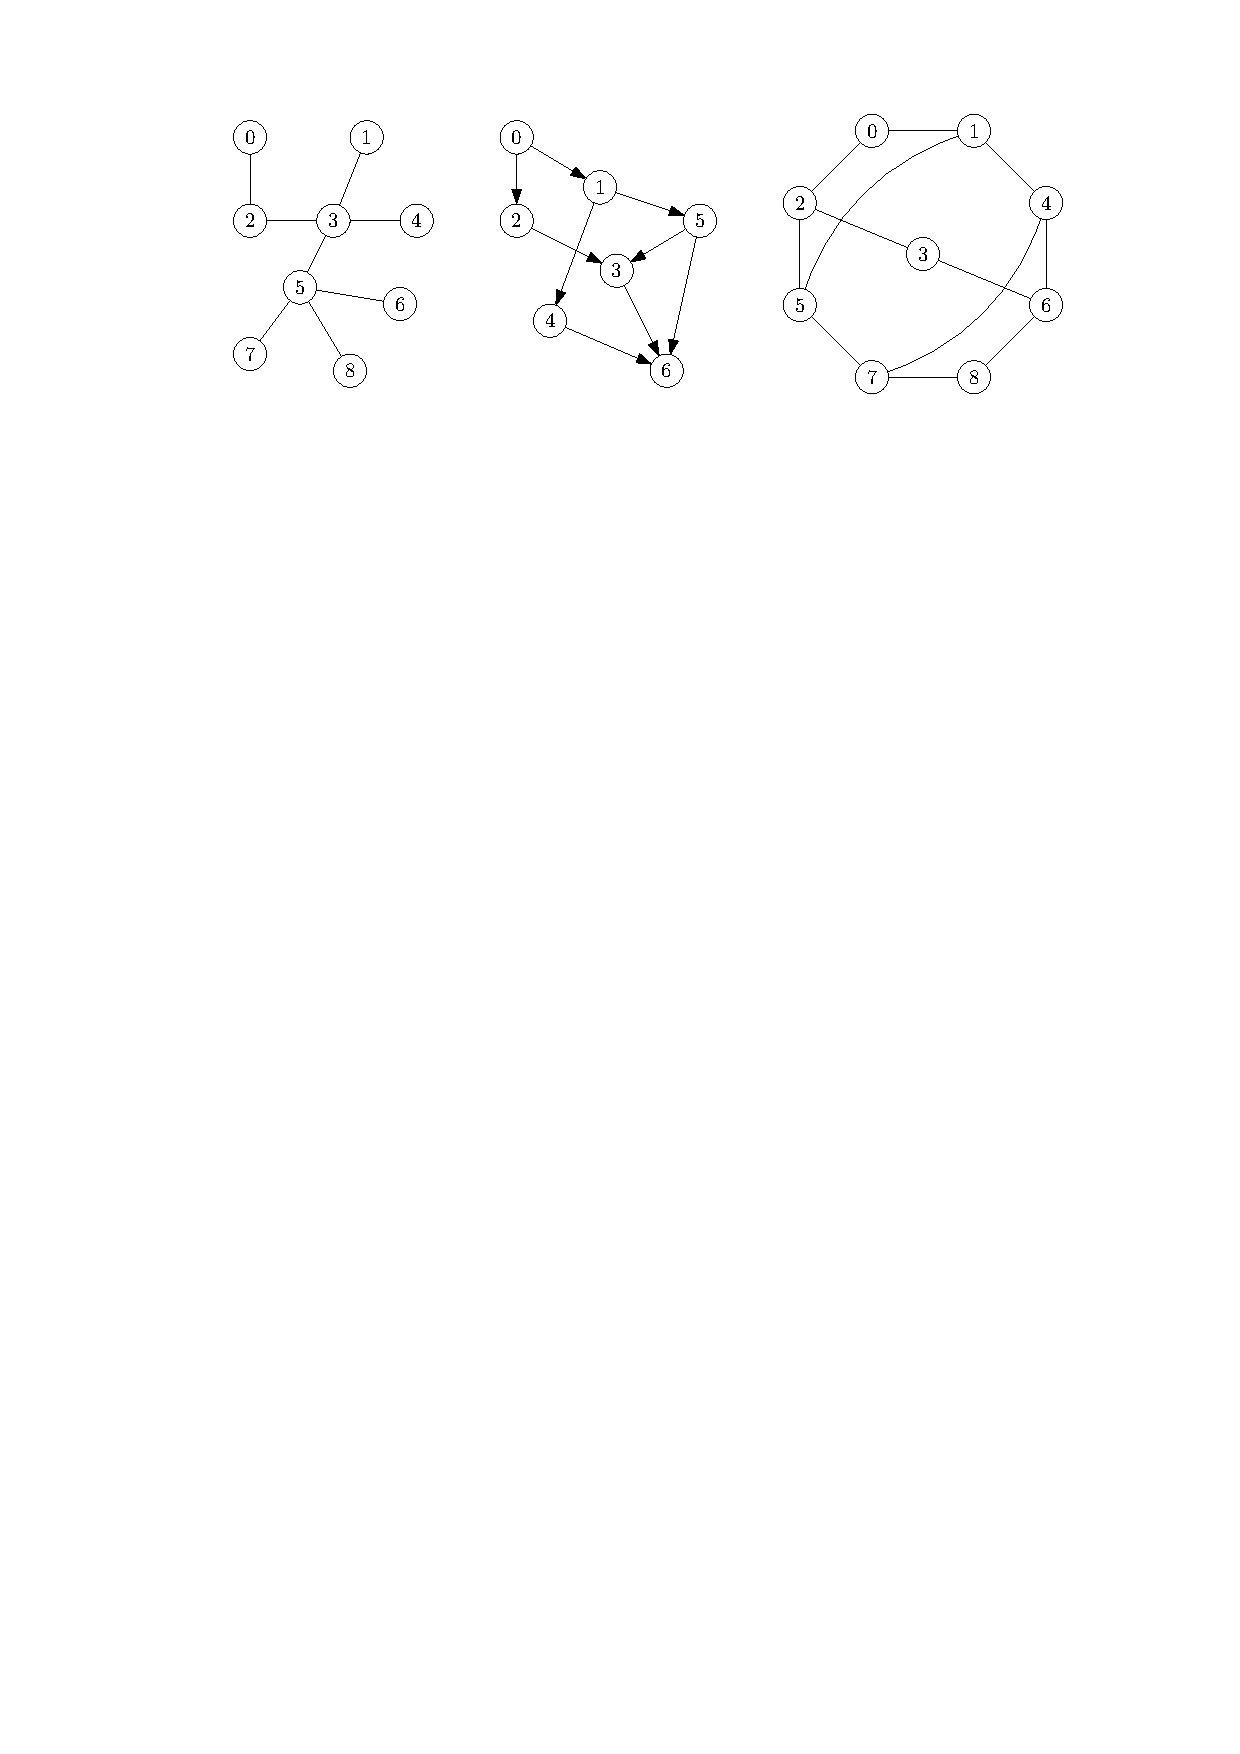
\includegraphics{graphEx3}
\caption{Some (di)graphs with different cycle behaviour.}
\label{fig:cycle}
\end{figure}

How to compute the girth of a graph? Here is an algorithm for finding
the length of a shortest cycle containing a given vertex $v$ in a graph
$G$. Perform \algfont{BFSvisit}. If we meet a grey neighbour (that is,
we are exploring edge $\{x, y\}$ from $x$ and we find that $y$ is already
grey), continue only to the end of the current level and then stop. For
each edge $\set{x, y}$ as above on this level, if $v$ is the lowest
common ancestor of $x$ and $y$ in the BFS tree, then there is a cycle
containing $x, y, v$ of length $l=d(x) + d(y) + 1$. Report the minimum
value of $l$ obtained along the current level.

\begin{Theorem}
\label{thm:BFS-cycle} 
The above algorithm is correct.
\end{Theorem}

\begin{proof}
Suppose that we arrive at vertex $x$, $d(x) = k$, and we have just
encountered a grey neighbour $y$. Then $d[y] = d[x] + 1$ or $d[y] = d[x]$
(note that $d[x] = d[y] + 1$ is ruled out because then $x$ would be a
child of $y$ and $y$ would be black). This means that there is definitely
a cycle containing $x, y$ and $z$, where $z$ is the lowest common ancestor
of $x$ and $y$ in the BFS tree. Note that $z\neq x, z\neq y$ since neither
$x$ nor $y$ is an ancestor of the other. The cycle consists of the tree
edges from $z$ to $x$, the cross edge $\set{x,y}$ and the tree edges
from $z$ to $y$. The length of the cycle is $l=d[x] + d[y] - 2 d[z] + 1$.

Conversely, let $C$ be any cycle and let $z$ be the first vertex of
the cycle reached by the search. Let $x$ and $y$ be two vertices in $C$
whose distance  from $z$ is greatest, with $d[x] \leq d[y]$. Then the
lowest common ancestor of  $x$ and $y$ is exactly $z$, and the cycle
found in the first paragraph is exactly $C$.

The vertex $v$ belongs to the cycle $C$ if and only if $v = z$. The
length of the cycle is $2k+1$ if $d[x] = d[y]$ and $2k+2$ if $d[y] =
d[x] - 1$. The minimum length of any cycle containing $v$ found after
this is $2(k+1) + 1 = 2k+3$, so no better cycle can be found after the
current level $k$ is explored.
\end{proof}

\begin{note}
An easy-to-implement DFS idea may not work properly. For example,
the DFS tree originating from vertex $0$ of the third graph of
\cref{fig:cycle} finds only $6$-cycles with the back edges (even
though a $4$-cycle exists using two of the back edges).
\end{note}

To compute the girth of a graph, we can simply run the above algorithm
from each vertex in turn, and take the minimum cycle length achieved.

\chapter{Bipartite graphs and matchings}


\subsection{Bipartite graphs}
\label{subsec:bipartite}

Many graphs in applications have two different types of nodes, and no
relations between nodes of the same type (this is a model of sexually
reproducing organisms, for example).

\begin{Definition}
A graph $G$ is \defnfont{bipartite} if $V(G)$  can be partitioned into
two nonempty disjoint subsets $V_0, V_1$ such that each edge of $G$
has one endpoint in $V_0$ and one in $V_1$.
\end{Definition}

\begin{Example}
The graph in \cref{fig:bipartite} is bipartite.  The isolated
vertex could be placed on either side.
\end{Example}

\begin{figure}
\centering
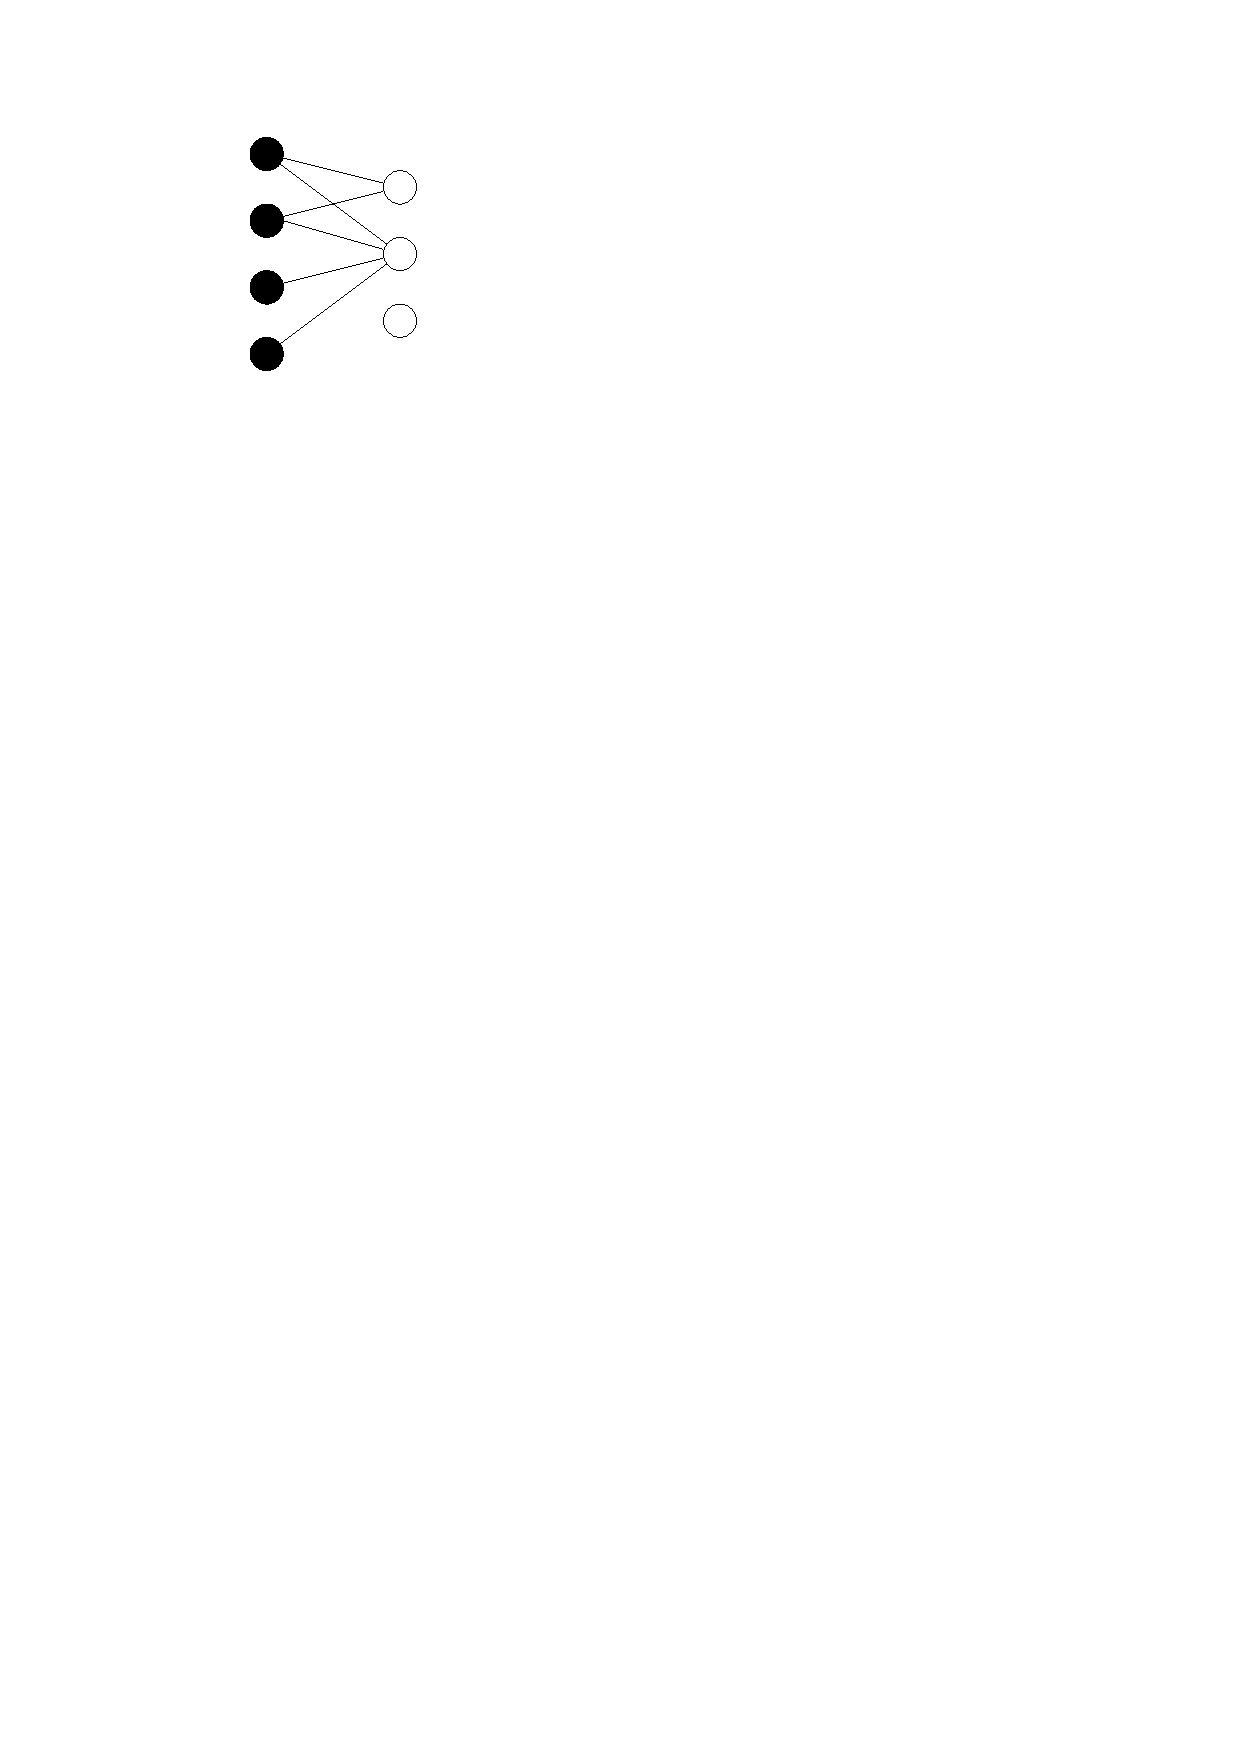
\includegraphics{bipartiteEx} 
\caption{A bipartite graph.}
\label{fig:bipartite}
\end{figure}

Showing that a graph is bipartite can be done by exhibiting a
\defnfont{bipartition} (a partition into two subsets as in the
definition). Of course finding such a bipartition may not be easy. Showing
a graph is not bipartite seems even harder. In each case, we certainly
do not want to have to test all possible partitions of $V$ into two
subsets! There is a better way.

\begin{Definition}
Let $k$ be a positive integer. A graph $G$ has a \defnfont{$k$-colouring}
if $V(G)$ can be partitioned into $k$ nonempty disjoint subsets such
that each edge of $G$ joins two vertices in different subsets.
\end{Definition}

\begin{Example}
The graph in \cref{fig:bipartite} has a 2-colouring as indicated.
\end{Example}

It is not just a coincidence that our example of a bipartite graph
has a 2-colouring.

\begin{Theorem} 
The following conditions on a graph $G$ are equivalent.
\begin{itemize}
\item
$G$ is bipartite;
\item
$G$ has a $2$-colouring;
\item
$G$ does not contain an odd length cycle.
\end{itemize}
\end{Theorem}

\begin{proof} 
Given a bipartition, use the same subsets to get a $2$-colouring, and
vice versa. This shows the equivalence of the first two conditions. Now
suppose $G$ is bipartite.  A cycle must have even length, since the start
and end vertices must have the same colour. Finally suppose that $G$
has no odd length cycle. A $2$-colouring is obtained as follows. Perform
BFS and assign each vertex at level $i$ the ``colour" $i \bmod 2$. If we
can complete this procedure, then by definition each vertex goes from
a vertex of one colour to one of another colour. The only problem could
be if we tried to assign a colour to a node $v$ that was adjacent to a
node $w$ of the same colour at the same level $k$. But then a cycle of
length $2k+1$ is created.
\end{proof}

It is now easy to see that we may use the method in the proof above
to detect an odd length cycle if it exists, and otherwise produce a
$2$-colouring of $G$. This of course runs in linear time.

\subsection*{Exercises}

\begin{Exercise}
\label{ex:shortest-cycle-thm}
Give an example to show that in the shortest cycle algorithm, if we
do not continue to the end of the level, but terminate when the first
cycle is found, we may find a cycle whose length is one more than the
shortest possible.
\end{Exercise}

\begin{Exercise}
\label{ex:shortest-cycle-runtime}
What is the time complexity of the shortest cycle algorithm?
\end{Exercise}

\begin{Exercise}
\label{ex:do2col}
The \defnfont{$n$-cube} (\defnfont{hypercube}) is a 
graph on $2^n$ vertices, each labelled by
a different bit vector of length $n$. If $\mathbf{v} = (v_0, \dots ,
v_{n-1})$ and $\mathbf{w} = (w_0, \dots , w_{n-1})$ are such bit vectors,
then there is an edge between the vertex labelled $\mathbf{v}$ and a
vertex labelled $\mathbf{w}$ if and only if $\mathbf{v}$ and $\mathbf{w}$
differ in exactly one component. For which values of $n$ is the $n$-cube
bipartite?
\end{Exercise}

\section{Maximum matchings}
\label{sec:matching}

Next we want to introduce an important graph problem that can
be solved in polynomial time by a clever path augmentation algorithm.  

\begin{Definition}
A \defnfont{matching} in a graph is a set of pairwise non-adjacent edges
(that is, each vertex can be in at most one edge of the matching).
A \defnfont{maximal matching} is a matching such that is not a proper subset
of any other matching.
A \defnfont{maximum matching} is one with the largest possible number of
edges (over all possible matchings).
\end{Definition}

Often, for many real-world problems, we want to find a maximum matching 
in bipartite graphs as illustrated by the next two examples.  

\begin{Example}
Suppose we have a set of workers $V_0$ and a set of tasks $V_1$ that need to be
assigned.  A given worker of $V_0$ is able to perform a subset of the tasks in $V_1$.
Now with each worker capable of doing at most one task at a time, the boss 
would like to assign (match) as many workers as possible to as many of 
the tasks. 
\end{Example}

\begin{Example}\label{ex:mp}
Consider the \defnfont{marriage problem} 
where we have a set of men and women (as vertices) and edges 
representing compatible 
relationships.  The goal is to marry as many couples
as possible, which is the same as finding a maximum matching in the
relationship graph.  If there are no homosexual interests then we have a 
bipartite graph problem.
\end{Example}

In \cref{fig:matchbipartite} we illustrate the difference between
a maximal and maximum matching in the setting of \cref{ex:mp}.
The matchings consist of bold-dashed edges (between females on the left
and males on the right) in the drawings.

\begin{figure}
\centering
\includegraphics{bipartiteMatching}
\caption{A maximal and maximum matching in a bipartite graph.}
\label{fig:matchbipartite}
\end{figure}

It is easy to find a maximal matching $M$ in a graph. For example, 
a simple greedy approach of
iterating over all edges and adding each edge to $M$ if it is
non-adjacent to anything already in $M$ will work.  As illustrated in
\cref{fig:matchbipartite}, a maximal matching may have fewer
edges than a more desirable maximum matching.

Our algorithm to compute a maximum matching will be based on
trying to improve an existing matching $M$ by finding certain
types of paths in a graph.

\begin{Definition}
Given a matching $M$, an \defnfont{alternating path} is a path in which 
the edges 
of the path alternate from being in the matching and not.
An \defnfont{augmenting path} is an alternating path that starts from and ends 
on unmatched vertices.
\end{Definition}

For example, consider the augmenting path Eve--Doug--Cher--Fred of
\cref{fig:matchbipartite}.  It contains three edges but only the
middle edge is part of a matching on the left case.  We can get the
better matching on the right if we add Eve-Doug, remove Doug--Cher, and add 
Cher--Fred to the existing matching.  Thus, in general, we see that we can 
improve a matching if we can find an augmenting path.  Note that there is always one
more non-matching edge than matching edge in an augmenting path.
Likewise, it is pretty easy to show that if there is no such augmenting path 
then we must have a maximum matching (see Exercise~\ref{ex:agpath}).

We next present a polynomal-time algorithm that finds an augmenting path if
one exists.  The basic idea is to start from an unmatched vertex $v$
and build a tree (via a graph traversal algorithm such as BFS) 
of alternating paths away from $v$.  If we reach another unmatched vertex 
then we have found an augmenting path.  Otherwise, if we visit all vertices
(in the same component as $v$) then we conclude that no augmenting 
path exists starting at $v$.  This algorithm is given in \cref{fig:augpath}.


%\begin{algorithm}[H]
%  \caption{An algorithm to find an augmenting path, given a matching
%and an unmatched starting vertex.}
%    \label{alg:augpath}
%\begin{algorithmic}[1]
%\Function{findAugmentingPath}{bipartite graph $G$; matching $M$; unmatched vertex $x$}
%	\State queue $Q$
%	\State array $\status[0..n-1]$, $\pred[0..n-1]$
%	\For{$u \in V(G)$}
%  		\State $\status[u] \gets $ WHITE; $\pred[u] \gets $ NULL 
%	\EndFor
%	\State $\status[x] \gets $ EVEN
%	\State $Q$.\algfont{insert}$(x)$
%	\While{\textbf{not}  $Q$.\algfont{isEmpty}$()$}
%		\State $u \gets Q$.\algfont{pop}$()$
% 		\If{$\status[u] =$ EVEN}
% 			\For{each $v$ adjacent to $u$}
% 				\If{$\status[v]$ = WHITE}
% 					\State $\status[v] \gets$ ODD; $\pred[v] \gets$ u
% 					\If{$v$ is unmatched in $M$}
% 						\State \Return{path $x,\ldots, \pred[\pred[u]], \pred[u], u, v$}
% 					\Else
%	 					\State $Q$.\algfont{insert}$(v)$
% 					\EndIf
% 				\EndIf
% 			\EndFor
% 		\Else 			\Comment{that is, $\status[u] =$ ODD} 
%			\State $v \gets$ matched vertex of $u$ from $M$
%			\If{$status[v]$ = WHITE}
%				\State$\status[v] \gets$ EVEN; $\pred[v] \gets u$
% 				\State$Q$.insert$(v)$
%	 		\EndIf
% 		\EndIf
%	\EndWhile
%	\State \Return{false} \Comment{no augmenting paths containing $x$}
%\EndFunction
%\end{algorithmic}
%\end{algorithm}



\begin{Theorem}
There exists a polynomial-time algorithm to find a maximum matching
in a bipartite graph.
\end{Theorem}
%\begin{proof}
%We first need to show that the algorithm \algfont{findAugmentingPath}, given in
%\cref{fig:augpath}, does find an augmenting path if one exists.
%It is sufficient to show that if there exists at least one augmenting path 
%from vertex $x$ to some other unmatched vertex that we find any one of them 
%(in our case, by imitating BFS, it will be one of shortest length).  
%\algfont{findAugmentingPath}
%builds a traversal tree starting at $x$ using the following constraints.
%\begin{itemize}
%\item If a reachable vertex $u$ is in the same partition as $x$ (status will
%be set to EVEN by the algorithm) then we know (except for $x$) that there is 
%an alternating path with the last edge including $u$ being in the matching.
%\item If a reachable vertex $v$ is not in the same partition as $x$ (status will
%be set to ODD if it is matched) then we know that there is 
%an alternating path with the last edge including $v$ is not in the matching.
%\end{itemize}
%This process produces a tree with alternating paths rooted at $x$ as 
%illustrated in \cref{fig:augtree}.  The status of the nodes are ODD 
%or EVEN depending if they are an even or odd distance from $x$.  If a vertex 
%(first seen) is at an odd distance then we have seen an alternating path 
%where the last edge is not in the matching.  If this last vertex is unmatched 
%then we have found an augmenting path, otherwise we extend the path by using 
%the matched edge.  
%If a vertex is at an even distance then we have seen an alternating path
%where the last edge is in the matching.  Since the graph is bipartite the
%status of being ODD or EVEN is unambiguous.
%
%\begin{figure}
%\centering
%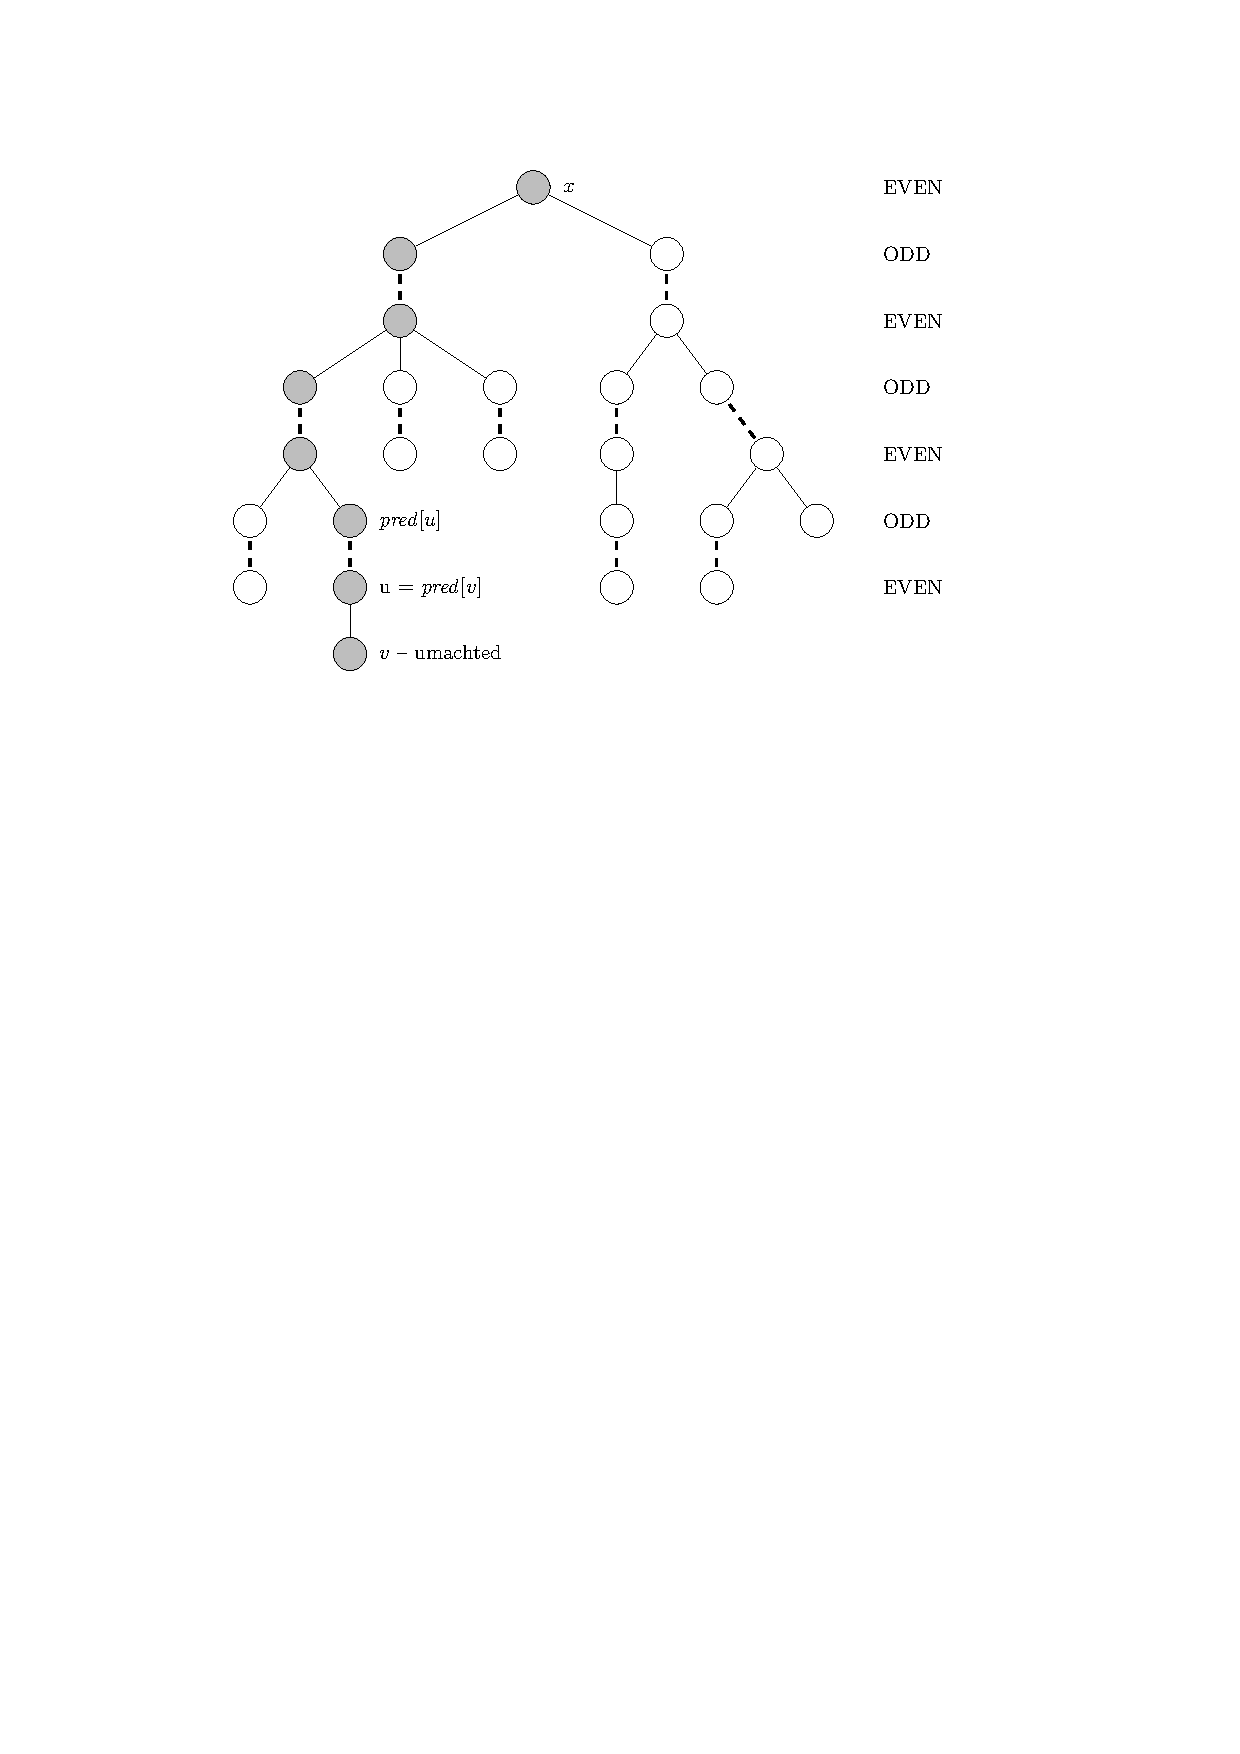
\includegraphics{augtree} 
%\caption{Structure of the graph traversal tree for finding augmenting paths.}
%\label{fig:augtree}
%\end{figure}
%
%Suppose the algorithm \algfont{findAugmentingPath} terminates without
%finding an augmenting path when one does exist.  Let $x=v_0,v_1,\ldots,v_k$
%be a counterexample.  Consider the
%first index $0<i\leq k$ such that $status[v_i] =$ WHITE.  We know $v_{i-1}$ was
%inserted in the queue $Q$. Consider the two cases.  If $i-1$ is even then
%since $v_i$ is a neighbour of $v_{i-1}$ its status would have changed to
%ODD.
%If $i-1$ is odd then either $(v_{i-1},v_i)$ is in the matching or not.
%If so, the status of $v_i$ would have changed; if not, a prefix of the 
%counterexample is not an augmenting path.  Thus, by contradiction,
%\algfont{findAugmentingPath} will find an augmenting path if one exists.
%
%The running time of one invocation of \algfont{findAugmentingPath} is the same 
%as the running time of BFS since each vertex is added to the queue $Q$
%at most once.  For adjacency list representation of graphs this 
%can be carried out in time $O(m)$.  If we find an augmenting path
%then our best matching increases by one.  
%Since a maximum matching is bounded by $\lfloor n/2 \rfloor$ we
%only need to find at most $O(n)$ augmenting paths.
%We potentially need to call \algfont{findAugmentingPath}
%once for each unmatched vertex, which is bounded by $O(n)$, and 
%repeat the process for each modified matching.  Therefore, the total 
%running time to find a maximum matching is at most $O(n^2m)$.
%\end{proof}

The algorithm presented here can easily be improved to $O(nm)$ by
noting that it is only required to traverse and compute an 
``alternating path forest'' in order to find an augmenting path.  
That is, we do not need to originate a call to \algfont{findAugmentingPath} for all 
unmatched vertices. However the correctness is a bit tricky to justify.

There are other algorithms that find maximum matchings more efficiently
than the one presented.  One of these is the Hopcroft-Karp algorithm
which runs in time $O(m\sqrt{n})$ and is based on finding a maximal 
flow in a network (by adding a source and sink vertex and directing all edges
from one vertex partition to the other of the bipartite graph).

We conclude this section by mentioning that there also exist
poly\-nomial-time algorithms to find maximum matchings in arbitrary
(non-bipartite) graphs. The details are beyond the scope of this book.

%\subsection*{Exercises}

\begin{Exercise}\label{ex:agpath}
Prove that a matching for a graph is maximum if and only if it does not
have any augmenting paths.
\end{Exercise}

\begin{Exercise}
Give an example of a bipartite graph of order 12 with a maximal matching 
that has an augmenting path of length 5 and a maximum matching of 
the same graph with two more edges.
\end{Exercise}

%\if 01
%\begin{Exercise}
%Explain what changes need to be done to the algorithm
% \algfont{findAugmentingPath} 
%so that it runs in time $O(|E|)$ and traverses all of the bipartite graph
%(instead of just the tree reachable from the unmatched vertex $x$).
%\end{Exercise}
%\fi

\begin{Exercise}\label{ex:konig}
Show that the size of a maximum matching in a bipartite graph $G=(V,E)$ is the
same as the size of the smallest \defnfont{vertex cover} of $G$.  A vertex cover
is a subset $V' \subseteq V$ of vertices such that for 
all $(u,v) \in E$, at least one of $u$ or $v$ is in $V'$.
Does the equality hold for arbitrary graphs?
\end{Exercise}

%\section{Notes}
%
%The linear-time algorithm for finding strong components of a digraph was 
%introduced by R. E. Tarjan in 1971.
%
%One of the early polynomial-time algorithms for finding
%maximum matchings in bipartite graphs is based on the Ford--Fulkerson 
%network flow algorithm \cite{FF56} from 1956.
%The first polynomial-time algorithm for finding a maximum matching in an 
%arbitrary graph was presented by J.~Edmonds \cite{Ed65} in 1965.

%[FF56]
%L. R. Ford and D. R. Fulkerson 
%"Maximal flow through a network". 
%\textit{Canadian Journal of Mathematics} \textbf{8} (1956), pp 399--404.

%[Ed65]
%J. Edmonds.  Paths, trees, and flowers
%\textit{Canadian Journal of Mathematics} \textbf{17} (1965), pp. 449-467. 
